\documentclass[11pt]{article}
\usepackage[utf8]{inputenc}
\usepackage{amssymb,amsmath,amsthm,mathtools,booktabs}
\usepackage[english]{babel}

\numberwithin{equation}{section}

\newtheorem{theorem}{Theorem}[section]
\newtheorem{corollary}{Corollary}[theorem]
\newtheorem{lemma}[theorem]{Lemma}

\topmargin -0.5in
\textheight 9.0in
\oddsidemargin  -0.05in
\evensidemargin -0.05in
\textwidth 6.5in
\renewcommand
\baselinestretch{1.0}

\newcommand{\tr}{{\text{tr}}}
\newcommand{\B}[1]{\textbf{#1}}
\newcommand{\T}[1]{\texttt{#1}}

\title{The Qudit Arthurs-Kelly Measurement}
\author{Matthew B. Weiss}

\begin{document}
\maketitle

\begin{abstract}
In this note we adapt the Arthurs-Kelly procedure for realizing Weyl-Heisenberg (WH) covariant POVM's to finite dimensional quantum systems. To perform such a POVM on a $d$-dimensional system, one prepares two $d$-dimensional ancillary systems in a particular initial state; subsequently,  the ancillas are  shifted coherently conditional on the position and momenta of the system of interest, and then measured. We discuss how to prepare the proper initial state of the ancillas from desired WH fiducial state, and for $d=2^n$ dimensional systems, we provide a decomposition of the qudit Arthurs-Kelly procedure into one and two qubit gates. Indeed, we provide a construction of qudit clock and shift operators (and their controlled counterparts) in terms of qubit operations. In particular, we specialize to the implementation of a SIC-POVM in $d=4$, exploiting the ``monomial representation'' of the WH group to prepare the SIC fiducial. We implement our constructions using Google's \T{cirq} framework, and run it on a realistic simulation of their Willow quantum chip. Using the same building blocks, we provide a dramatically simpler implementation of a WH-POVM using a single $d$-dimensional ancilla: the cost is that the system is projected into a computational basis state afterwards. We extend our results to all dimensions which are a power of 2, using a state preparation ansatz to prepare the SIC fiducial states.
\end{abstract}


\section{Introduction}

In 1965, Arthurs and Kelly \cite{ArthursKelly, PhysRevA.43.1153} proposed a realization of the canonical coherent state measurement using the following scheme. Two ancilla systems begin in Gaussian states centered at the origin of the infinite line; the ancillas are then coupled to a system of interest such that system's position drives translations of the first ancilla, and the system's momentum drives translations of the second ancilla. Upon position measurements of the two ancillas, by analyzing the resulting Kraus operators, it is possible to show that one ought to project the system state into a coherent state with the appropriate probability. Recall that the coherent states may be obtained as the orbit of the vacuum state under the Weyl-Heisenberg (WH) group. In fact, the Arthurs-Kelly procedure may realize more general WH-covariant measurements for different choices of initial states for the ancillas.

 In this note, we show how the Arthurs-Kelly measurement may be adapted to finite dimensional systems, or qudits. In the case that $d=2^n$, we provide a program for decomposing the required qudit operations into one and two qubit operations. One special class of finite-dimensional WH-covariant measurements are SIC-POVMs (symmetric informationally-complete) \cite{Renes_2004}: a SIC's $d^2$ rank-1 POVM elements may be rescaled into pure states which form a regular simplex inscribed in quantum state-space, and in all save one sporadic case, SICs are covariant under the discrete WH group \cite{Stacey2021}. In particular, we specialize to the implementation of a  SIC in dimension four. We also show how, if one is willing to sacrifice the post-measurement projection onto a SIC state, one may realize a WH-POVM in a considerably simpler way. Finally, using a state preparation ansatz, we extend our results to any power of 2 dimension. 

\section{Weyl-Heisenberg operators}

Fixing a Hilbert space $\mathcal{H}_d$, let clock and shift operators \cite{Gross_2021} be defined as
\begin{align}
Z|m\rangle = \omega^{m}|m\rangle && 	X|m\rangle = |m+1\rangle
\end{align}
where $\{|m\rangle\}_{m=0}^{d-1}$ denote  discrete position states (which we may take to be the computational basis states) and $\omega=e^{2\pi i/d}$. Note that all addition is understood mod $d$. The clock and shift  operators satisfy the relation $ZX=\omega XZ$, and we may use them to define a representation (up to phase) of the group $\mathbb{Z}_d\times \mathbb{Z}_d$ in terms of Weyl-Heisenberg (WH) displacement operators
\begin{align}
D_{\B{a}}=X^{a_1}Z^{a_2} && \B{a}=(a_1, a_2)\in \mathbb{Z}_{d}^2.
\end{align}
Some fundamental properties of these operators include
\begin{align}
D_\B{a}&=\omega^{-a_1a_2}Z^{a_2} X^{a_1} \\
D_\B{a}^\dagger &= \omega^{a_1a_2}D_{-\B{a}}\\
D_\B{a}D_\B{b}&=\omega^{a_2b_1}D_{\B{a}+\B{b}}\\
D_{\B{b}}^\dagger D_\B{a}D_{\B{b}} &= \omega^{a_2b_1-a_1b_2}D_{\B{a}}\\
\tr(D_{\B{a}}^\dagger D_\B{b})&=d\delta_{\B{a}\B{b}},
\end{align}
which may be confirmed by straightforward calculation.
The last shows that the WH operators form an orthonormal operator basis so that we may write any operator as
\begin{align}
O &= \frac{1}{d}\sum_\B{a}\tr(D_\B{a}^\dagger O)D_\B{a}.
\end{align}

Since $Z=\sum_m \omega^{m}|m\rangle\langle m|$, we may define a discrete position operator $Q=\sum_m \frac{2\pi m}{d}|m\rangle\langle m|$ such that $Z = e^{iQ}$. Let $F=\frac{1}{\sqrt{d}}\sum_{jk}\omega^{jk}|j\rangle\langle k|$ be the discrete Fourier transform operator. We may define discrete momentum states as $|m\rangle_p=F|m\rangle=\frac{1}{\sqrt{d}}\sum_j\omega^{jm}|j\rangle $, so that $\langle k|m\rangle_p=\frac{\omega^{km}}{\sqrt{d}}$. In fact, $X=F^\dagger Z F$ from which it follows that $X=\sum_m \omega^{-m}|m\rangle_p\langle m|_p$ and if we define the discrete momentum operator $P=\sum_m \frac{2\pi m}{d}|m\rangle_p\langle m|_p$, then $X=e^{-iP}$. Finally, we note that just as $X$ shifts position states, $Z$ shifts momentum states, $Z|m\rangle_p=|m+1\rangle_p$.



\section{SIC-POVMs}

A SIC is a set $\{\Pi_i\}_{i=1}^{d^2}$ of rank-1 projectors on $\mathcal{H}_{d}$ such that 
\begin{align}
\label{sic-condition}
	\tr(\Pi_i\Pi_j)=\frac{d\delta_{ij}+1}{d+1}.
\end{align}
Such projectors may be rescaled as $E_i = \frac{1}{d}\Pi_i$ so that $\sum_i E_i=I$, thereby furnishing a generalized measurement or POVM---in fact, such a measurement will be informationally complete since the SIC projectors form a basis for operators on $\mathcal{H}_d$. One may consider the orbit of a generic fiducial state $\Pi$ under the WH group, $\Pi_\B{a}=D_\B{a}^\dagger \Pi D_{\B{a}}$, and obtain a WH-covariant POVM. Only for a very special choice of projector, however, will Eq.\! \ref{sic-condition} be satisfied, and the set be symmetric informationally-complete (SIC). 


\section{Naimark dilation theorem}

By the Naimark dilation theorem \cite{Nielsen_Chuang_2010}, any POVM can be realized by entangling a system of interest with an ancilla system via a unitary interaction, and subsequently performing a standard measurement (PVM) upon the ancilla.  Let the overall Hilbert space be $\mathcal{H}_{d_A}\otimes \mathcal{H}_{d_S}$, where $d_A$ is the dimension of the ancilla, and $d_S$ is the dimension of the system. If the ancilla begins in the state $\sigma$, the system begins in the state $\rho$, the unitary interaction is denoted $U$, and the projector corresponding to the $i$th outcome of the measurement on the ancilla is $\Pi_i$, then the subsequent state of the system after the interaction and conditional on obtaining  outcome $i$ on the ancilla, ought to be
\begin{align}
\rho_i^\prime \propto \tr_A\Big( (\Pi_i \otimes I) U(\sigma \otimes \rho)U^\dagger (\Pi_i \otimes I)\Big),	
\end{align}
where $\tr_A$ denotes the trace over the ancilla degrees of freedom, and one normalizes by the probability of obtaining the outcome. Let us assume for simplicity that the initial state of the ancilla is pure $\sigma=|\gamma\rangle\langle \gamma|$, and the $\Pi_i$'s  correspond to projectors onto computational basis states $\Pi_i=|i\rangle\langle i|$. Then one may show that
\begin{align}
\rho_i^\prime = \frac{K_i \rho K_i^\dagger}{\tr(K_i^\dagger K_i \rho)} && K_i = \Big(\langle 	i| \otimes I\Big)U\Big(|\gamma\rangle \otimes I\Big),
\end{align}
where the $K_i$'s are Kraus operators acting on the system degrees of freedom only, and $K_i^\dagger K_i = E_i$ are POVM elements.

\section{Qudit Arthurs-Kelly}

Suppose we have assigned a total Hilbert space  $\mathcal{H}_d \otimes \mathcal{H}_d \otimes \mathcal{H}_d$, where the first two tensor factors corresponds to two ancillas, and the third to the system of interest. After preparing the ancillas according to an initial state $|\gamma\rangle$, we perform two unitaries in sequence: 1) a (leftward) shift of the first ancilla conditional on the discrete position of the system, 2) a (leftward) shift on the second ancilla conditional on the discrete momentum of the system. In other words, 
\begin{align}
U &= \left(\sum_m I \otimes X^{-m} \otimes |m\rangle_p\langle m|_p	\right)\left(\sum_k X^{-k} \otimes I \otimes |k\rangle\langle k|\right)\\
&=\frac{1}{\sqrt{d}}\sum_{km}\omega^{-km} X^{-k} \otimes X^{-m} \otimes |m\rangle_p\langle k|.
\end{align}
If we subsequently perform discrete position  measurements on the two ancillas, we obtain Kraus operators
\begin{align}
K_{xy}&=	\Big(\langle x, y|\otimes I\Big)U\Big(|\gamma\rangle \otimes I\Big) \\
&=\frac{1}{\sqrt{d}}\sum_{km}\omega^{-km}\langle x, y|X^{-k}\otimes X^{-m}|\gamma \rangle \ |m\rangle_p\langle k|\\
&=\frac{1}{\sqrt{d}}\sum_{km}\omega^{-km}\langle x+k, y+m|\gamma \rangle \ |m\rangle_p\langle k|.
\end{align}
Let us examine in particular the Kraus operator corresponding to the outcome $x=y=0$,
\begin{align}
	K_{00}&=\frac{1}{\sqrt{d}}\sum_{km}\omega^{-km}\langle k,m|\gamma\rangle \ |m\rangle_p\langle k|.
\end{align}
If we conjugate $K_{00}$ by a WH displacement operator $D_\B{a}$, we find
\begin{align}
	D_\B{a}^\dagger K_{00}D_\B{a}&=\frac{1}{\sqrt{d}}\sum_{km}\omega^{-km}\langle k,m|\gamma\rangle \ D_\B{a}^\dagger|m\rangle_p\langle k| D_\B{a}.
\end{align}
Letting $\B{a}=(x, y)$, we have
\begin{align}
	D_\B{a}^\dagger |m\rangle_p\langle k|D_\B{a} &= \omega^{xy}X^{-x}Z^{-y}|m\rangle_p\langle k| X^xZ^y\\
	&=\omega^{xy} X^{-x}|m-y\rangle_p\langle k -x|Z^{y}\\
	&=\omega^{xy}\omega^{x(m-y)}|m-y\rangle_p\langle k-x|\omega^{y(k-x)}\\
	&=\omega^{xy+xm-yx+yk-xy}|m-y\rangle_p\langle k-x|\\
	&=\omega^{-xy+xm+yk}|m-y\rangle_p\langle k-x|,
\end{align}
so that subtituting $a=k-x$ and $b=m-y$, we find
\begin{align}
D_\B{a}^\dagger K_{00}D_\B{a}&=	\frac{1}{\sqrt{d}}\sum_{km}\omega^{-km}\langle k,m|\gamma\rangle \ \omega^{-xy+xm+yk}|m-y\rangle_p\langle k-x|\\
&=\frac{1}{\sqrt{d}}\sum_{ab}\omega^{-(a+x)(b+y)}\langle x+a,y+b|\gamma\rangle \ \omega^{-xy+x(b+y)+y(a+x)}|b\rangle_p\langle a|\\
&=\frac{1}{\sqrt{d}}\sum_{ab}\omega^{-ab}\langle x+a,y+b|\gamma\rangle \ |b\rangle_p\langle a|\\
&= K_{xy}.
\end{align}
We conclude that we may obtain the whole set of Kraus operators by considering the orbit of $K_{00}$ under the WH group, and thus the corresponding measurement is a WH-covariant POVM. Which measurement is realized, however, depends on the initial state of the ancillas. Let $\Pi$ be the desired fiducial state. Let us assume that it is a rank-1 projector, and that we want the post-measurement update to be a projection by this same projector. Since we require $E_{00}=K_{00}^\dagger K_{00}=\frac{1}{d}\Pi$, we must have
\begin{align}
\Pi = \sum_{km}\omega^{-km}\langle k,m|\gamma\rangle \ |m\rangle_p\langle k| = \sum_{km}\langle m|_p\Pi|k\rangle \  |m\rangle_p\langle k|,
\end{align}
where on the RHS we've simply expanded the projector $\Pi$ by inserting the two resolutions of the identity provided by the position and momentum states in turn. Therefore the components of the ancillas in the position basis must be
\begin{align}
\label{ancilla}
	\langle k,m|\gamma\rangle=\omega^{km}\langle m|F^\dagger \Pi |k\rangle.
\end{align}
 For an alternate interpretation of this procedure, see appendix \ref{alt-interpretation}, and for a slight simplification see appendix \ref{slight-simplification}. We note that a similar method was proposed in \cite{10.1063/1.1827924,10.1063/1.2222080}.

\subsection{Preparing the ancillas}

Given a choice of fiducial state $\Pi$, Eq. \!\ref{ancilla} tells us what the initial state of the ancillas ought to be in order to realize the corresponding WH-covariant POVM. We now show how one can parlay the ability to prepare the fiducial state itself (and its complex conjugate) into the ability to appropriately prepare the ancillas. Suppose the desired fiducial is $\Pi = |\phi\rangle\langle \phi|$. Then: 1) the first ancilla is prepared according to $|\phi^*\rangle$ while the second is prepared according to $|\phi\rangle$; 2) the second ancilla is inverse Fourier transformed; 3) finally, the position of the first ancilla drives coherent rephasing of the second ancilla. Afterwards, the two ancillas will be in the desired initial state $|\gamma\rangle$ which realizes the WH-POVM  with fiducial $\Pi$. 
\begin{align}
\label{ancilla-prep}
\langle k, m|\left(\sum_j |j\rangle\langle j|\otimes Z^j	\right)\Big(I \otimes F^\dagger\Big)\Big(|\phi^*\rangle \otimes |\phi\rangle\Big) &=\sum_j \langle k|j\rangle \langle j|\phi^*\rangle \langle m|Z^jF^\dagger|\phi\rangle\\
&=\langle m|Z^k F^\dagger|\phi\rangle\langle \phi|k\rangle\\
&=\omega^{km}\langle m|F^\dagger \Pi |k\rangle.
\end{align}
For further intuition as to why this works,  see appendix \ref{alt-interpretation}, as well as section \ref{simplifiedWH}, and appendix \ref{operatorD}.

\section{A $d=4$ SIC fiducial}

According to \cite{monomial}, when $d=n^2$ is a square, an alternative representation of $X$ and $Z$ exists whereby not only elements of the Weyl-Heisenberg group, but also elements of its normalizer, the Clifford group, are represented by phase-permutation (or monomial) matrices. The transformation effecting the basis change from the standard basis to the ``monomial representation'' is simply $F_n \otimes I$, where $F_n$ is the $n\times n$ Fourier matrix. In particular, this representation often allows SIC fiducials to take unusually simple forms. When $d=4$, one simple example, adapted from Section 6 of \cite{monomial}, is as follows. Since $F_2=F_2^\dagger = H$ (the Hadamard transformation), one may check that
\begin{align}
\label{fiducial}
|\phi\rangle = 	(H \otimes I)\begin{pmatrix}1 & 0 & 0 & 0\\ 0 & e^{i\pi(-1/4)} & 0 & 0 \\ 0 & 0 & e^{i\pi (1/4)} & 0 \\ 0 & 0 & 0 & e^{i\pi (1/2)}\end{pmatrix}\frac{1}{\sqrt{5+\sqrt{5}}}\begin{pmatrix} \sqrt{2+\sqrt{5}} \\ 1 \\ 1 \\ 1 \end{pmatrix}
\end{align}
is a SIC fiducial with respect to the standard representation of $X$ and $Z$. Notice that the only non-trivial number that appears in this expression is $\sqrt{2+\sqrt{5}}$. Finally, we note that the diagonal phase matrix used in this expression (call it $P$) is the only place that complex components appear so that $|\phi^*\rangle$ can be prepared by acting with $P^\dagger$.

\section{Qubit implementation}

We now assume that $d=2^n$ for $n$ qubits. In order to realize the qudit Arthurs-Kelly measurement in term of qubit operators, we need three basic gates: the Hadamard ($\T{H}$), a controlled phase gate $\T{CR}(k)$, and the swap gate $\T{SWAP}$:
\begin{align}
\T{H}= \frac{1}{\sqrt{2}}\begin{pmatrix}1 & 1 \\ 1 & -1\end{pmatrix}	&&\T{R}(k) &= \begin{pmatrix}1 & 0 \\ 0 & e^{2\pi i/2^k} \end{pmatrix}
\end{align}
\begin{align}
\T{CR}(k) &= \begin{pmatrix}I & 0 \\ 0 & R(k)\end{pmatrix} && \T{SWAP} = \begin{pmatrix} 1 & 0 & 0 & 0\\ 0 & 0 & 1 & 0 \\ 0 & 1 & 0 & 0 \\ 0 & 0 & 0 & 1\end{pmatrix}.
\end{align}
We note that Google's \T{cirq} natively provides the  $\T{H}$ and $\T{SWAP}$ gates, and that $\T{R}(k)$ may be obtained from $\T{ZPowGate(exponent=}2^{1-k}\T{)}$,  its controlled counterpart being $\T{CZPowGate(exponent=}2^{1-k}\T{)}$.

The first observation is that the qudit Fourier transform $\T{F}$ can be realized as a sequence of Hadamards and controlled phase shifts ($\T{CR}$), followed by a sequence of $\T{SWAP}$'s at the end which reverse the order of the qubits \cite{Nielsen_Chuang_2010}:
\begin{center}
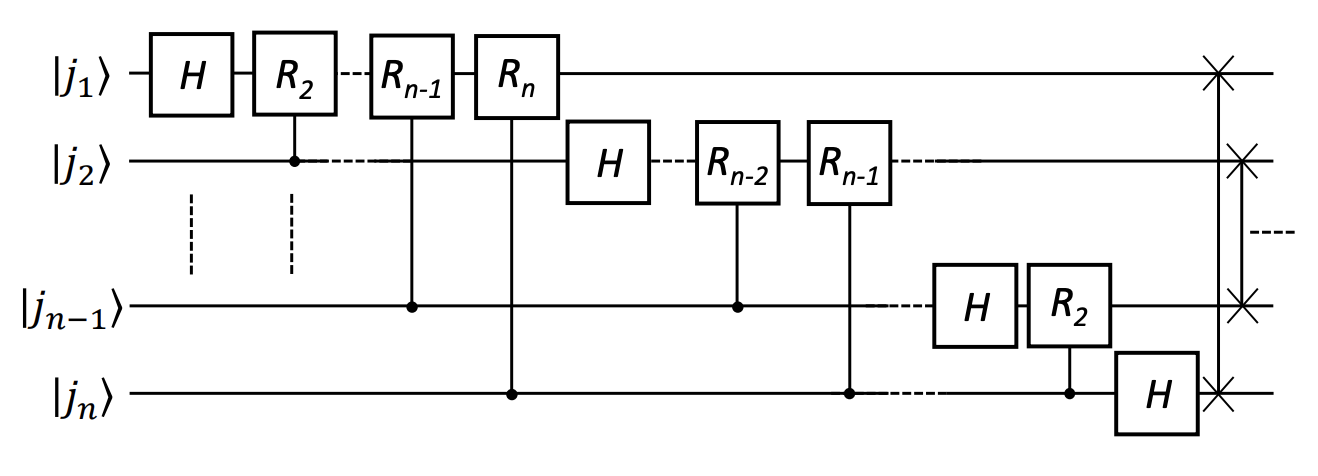
\includegraphics[scale=0.45]{img/qft.png}
\end{center}
Meanwhile, the qudit ($d=2^n$) clock and shift operators on $n$ qubits indexed by $\{q_j\}_{j=0}^{n-1}$ may be constructed as
\begin{align}
\T{Z}= \prod_{j=0}^{n-1} \T{R}_{q_j}(j+1) && \T{X}=\T{F}^\dagger \T{Z}\T{F}.
\end{align}
 Here $\T{R}_{q_j}$ denotes $\T{R}$ applied to the $q_j$'th qubit, and products ought to be understood from right to left. It is easiest to see that this works by direct calculation, e.g. for two qubits ($d=2^2=4$),
\begin{align}
\T{R}(1)\otimes \T{R}(2)
&= \begin{pmatrix} 1 & 0 \\ 0 & e^{\pi i }\end{pmatrix} \otimes   \begin{pmatrix} 1 & 0 \\ 0 & e^{\pi i/2}\end{pmatrix} 
	\\
&=\begin{pmatrix}1 & 0 & 0 & 0\\
0 &e^{\pi i /2} & 0 & 0 \\
0 & 0 & e^{\pi i } & 0 \\
0 & 0 & 0 & e^{3\pi i  /2} \end{pmatrix}\\
&=\sum_m e^{2\pi i m/4}|m\rangle\langle m|=\T{Z}.
\end{align}
Next, we need controlled counterparts of these operators. We first construct a qubit-controlled $\T{Z}$ operator,
\begin{align}
\T{QCZ}_{c,t} &= 	\prod_{j=0}^{n-1} \T{CR}_{c,t_j}(j+1),
\end{align}
which performs $\T{Z}$ on $n$ qubits indexed by $\{t_i\}_{i=1}^n$ conditional on the state of a control qubit $c$. For example, $\T{QCZ}$ on $1+3$ qubits:
\begin{center}
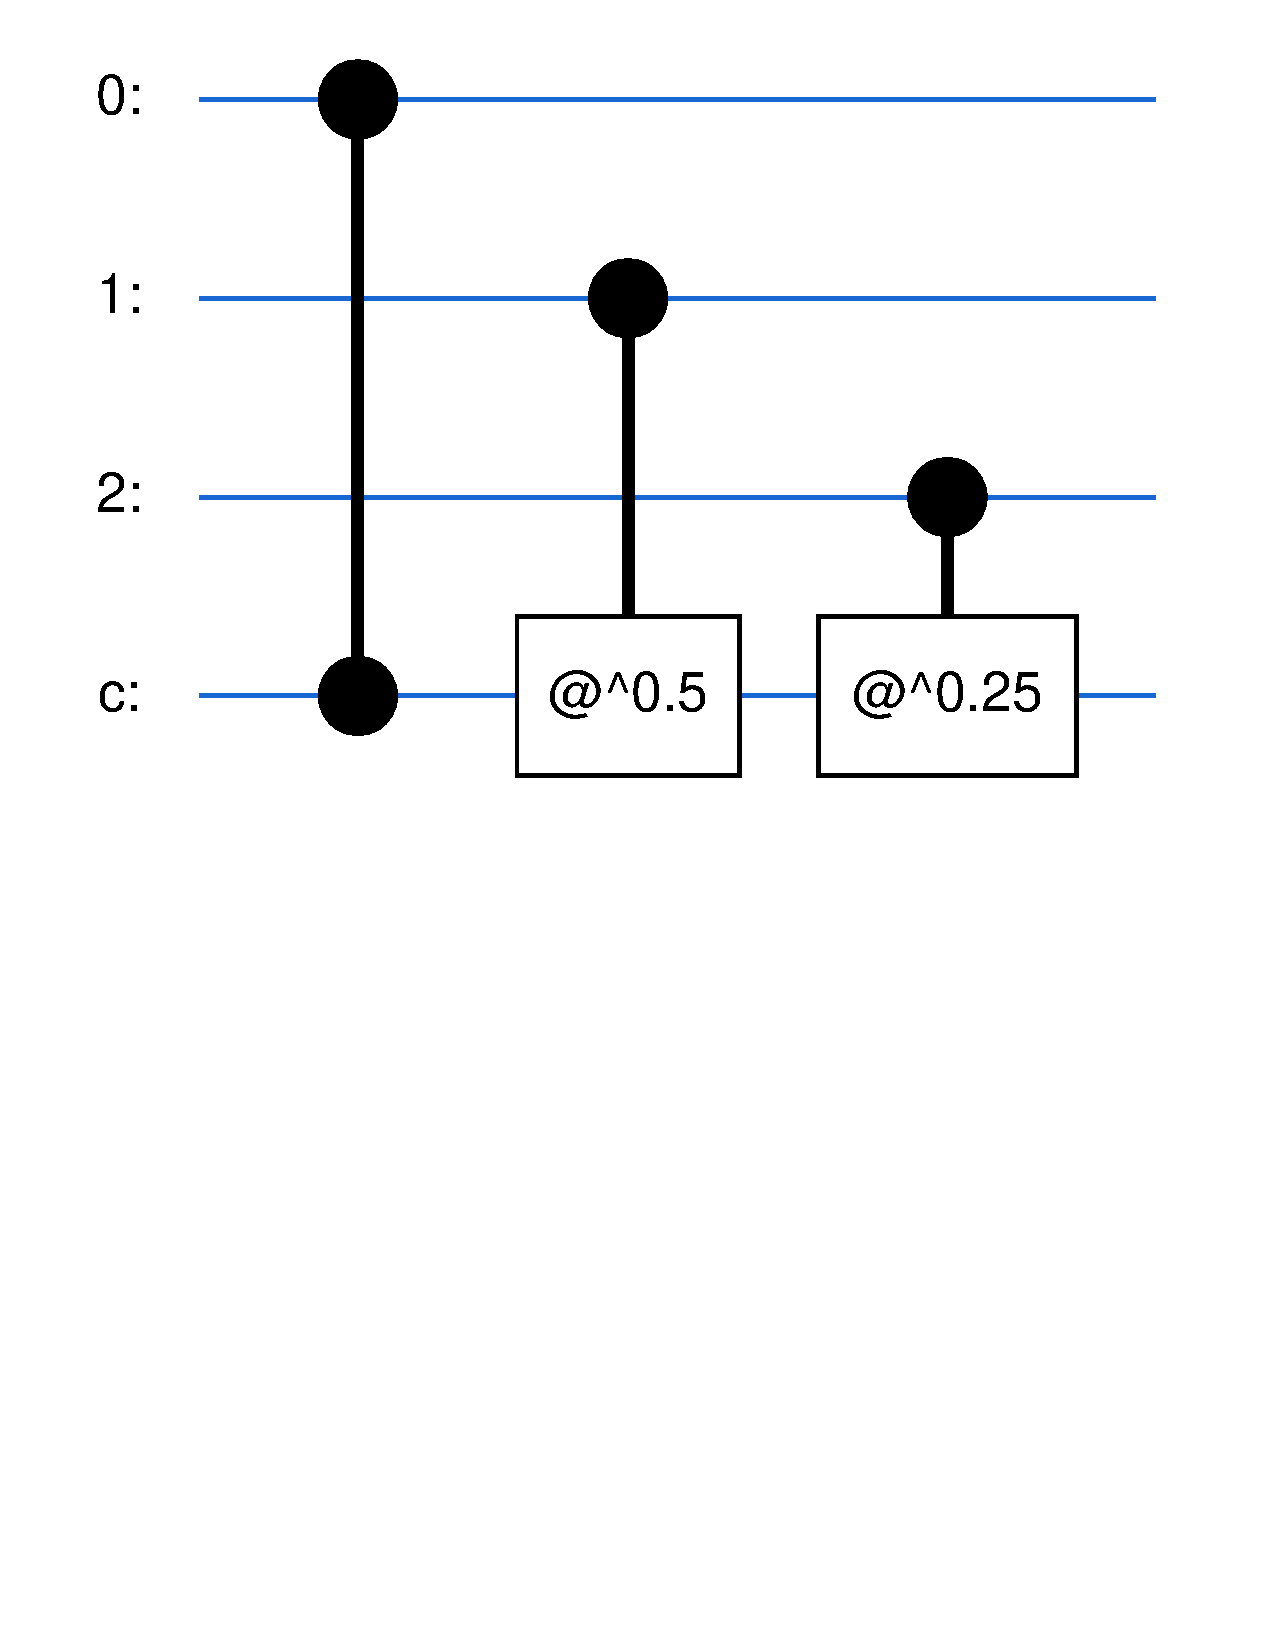
\includegraphics[scale=0.34]{img/qubit_controlled_clock.pdf}
\end{center}
The full qudit-controlled $\T{Z}$ operator, which performs $Z^k$ conditional on the control qudit being in the $|k\rangle$ state, may then be constructed as
\begin{align}
\T{CZ}_{c, t}	=\prod_{j=0}^{n-1} \T{QCZ}^{2^{j}}_{c_{n-j-1, t}},
\end{align}
where the control qudit is realized by $n$ qubits indexed by $\{c_j\}_{j=0}^{n-1}$, and the target qudit is realized by $n$  qubits indexed by $\{t_j\}_{j=0}^{n-1}$.  For example, $\T{CZ}$, where the first three qubits constitute the target qudit, and the second three qubits constitute the control:\begin{center}
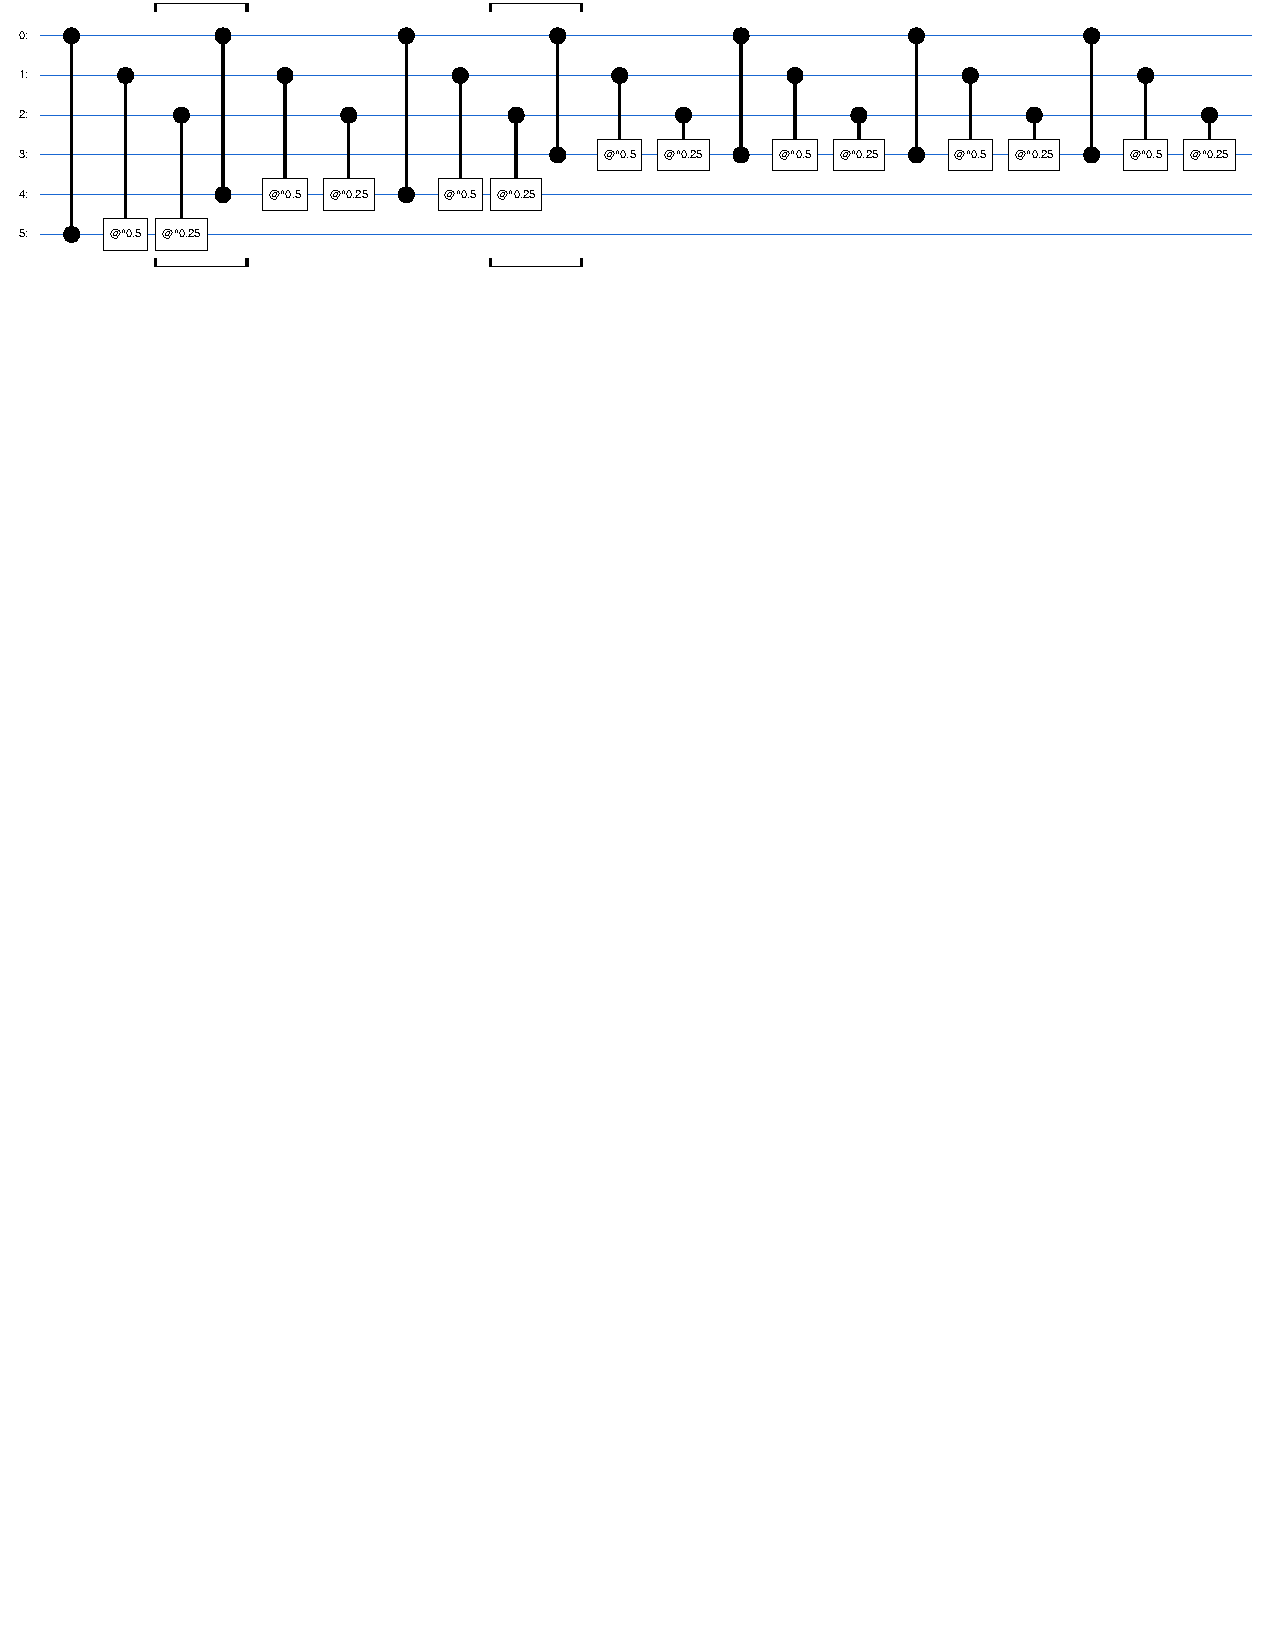
\includegraphics[scale=0.8]{img/controlled_clock.pdf}
\end{center}
Again, the logic is easiest to see by examining a simple case. Let $n=3$, and take the first three qubits to be the target, and the second three to be the control. Denoting $|0\rangle\langle 0| \equiv 0$ and $|1\rangle\langle 1 | \equiv 1$ and suppressing the tensor product sign, e.g. \!$ZII1=Z \otimes I \otimes I \otimes |1\rangle\langle 1| $, where the first tensor factor is a $2^3=8$ dimensional qudit, and the latter three tensor factors are treated as qubits,
\begin{align}
\T{CZ}_{c,t}&=\T{QCZ}^{2^2}_{0, t}\T{QCZ}^{2^1}_{1, t}\T{QCZ}^{2^0}_{2,t}\\
&=\Big(I0 II + Z^41II\Big)\Big(II0I+Z^2I1I\Big)\Big(III0+ZII1\Big) \\
&=\Big(I00I+Z^201I+Z^410I+Z^611I\Big)\Big(III0 + ZII 1\Big)\\
&=I000+Z001+Z^2010+Z^3011+Z^4100+Z^5101+Z^6110+Z^7111\\
&= \sum_{m=0}^{7}Z^m \otimes |m\rangle\langle m| .
\end{align}
Finally, $\T{CX}$ can be constructed by first applying $\T{F}$ to the target qubits, then $\T{CZ}$, followed by $\T{F}^\dagger$ on the target qubits. The Arthurs-Kelly unitary can then be expressed,
\begin{align}
\T{AK}= \T{F}_c\T{CX}_{c, t^{(2)}}^\dagger  \T{F}^\dagger_c \T{CX}^\dagger _{c,t^{(1)}}, 
\end{align}
where $c$ denotes the set of qubits realizing the qudit system of interest, and $t^{(1)}$ and $t^{(2)}$ are the two sets of qubits acting as ancillas. The first ancilla is shifted coherently (leftward) conditional on the position of the system; then the second ancilla is shifted coherently (leftward) conditional on the momentum of the system (hence the Fourier transforms). In circuit form, specializing to the case that $n=2$, where the first qubit pair is ancilla 1, the second qubit pair is ancilla 2, and the third qubit pair is the system of interest, we have:
\begin{center}
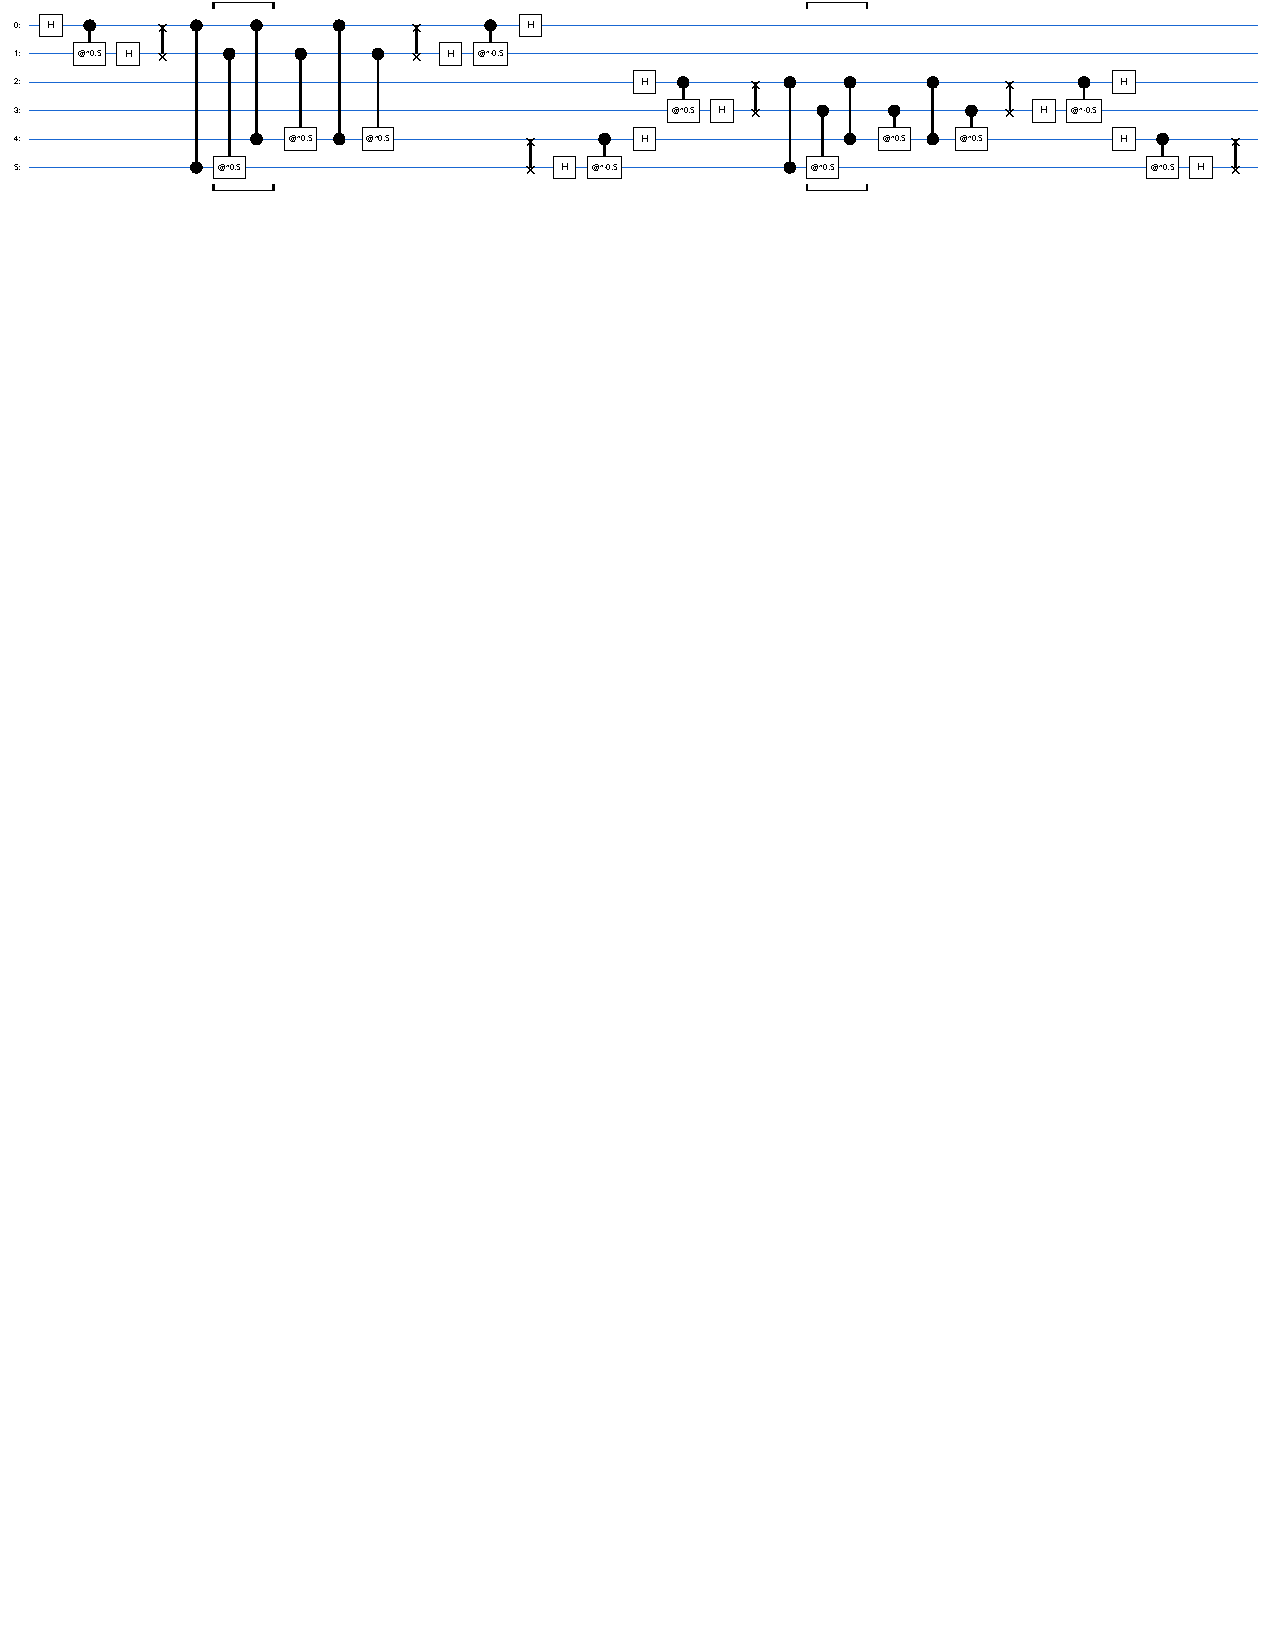
\includegraphics[scale=0.8]{img/ak.pdf}	
\end{center}

Finally, suppose that $\Pi = |\phi\rangle\langle \phi|$ is the WH fiducial state. Assuming that ancilla 1 ($t^{(1)}$) is prepared according to $|\phi^*\rangle$ and ancilla 2 ($t^{(2)}$) is prepared according to $|\phi\rangle$, following Eq. \!\ref{ancilla-prep}, we must apply the unitary
\begin{align}
	\T{AP}= \T{CZ}_{t^{(1)}, t^{(2)}}\T{F}^\dagger_{t^{(2)}}
\end{align}
to ready the ancillas for the Arthurs-Kelly procedure.

\subsection{Preparing the $d=4$ fiducial}
As we saw in Eq. \!\ref{fiducial}, an example of a SIC fiducial in $d=4$ is provided by 
\begin{align}
|\phi\rangle = 	(H \otimes I)\begin{pmatrix}1 & 0 & 0 & 0\\ 0 & e^{i\pi(-1/4)} & 0 & 0 \\ 0 & 0 & e^{i\pi (1/4)} & 0 \\ 0 & 0 & 0 & e^{i\pi (1/2)}\end{pmatrix}\frac{1}{\sqrt{5+\sqrt{5}}}\begin{pmatrix} \sqrt{2+\sqrt{5}} \\ 1 \\ 1 \\ 1 \end{pmatrix}.
\end{align}
In order to realize $|\phi\rangle$, we need the following gates:
\begin{align}
\T{Ry}(\theta)&= \begin{pmatrix}\cos (\theta/2) & -\sin(\theta/2) \\ \sin(\theta/2) & \cos (\theta/2) \end{pmatrix} && \T{Ph}(\theta)=\begin{pmatrix} 1 & 0 \\ 0 & e^{i \theta}\end{pmatrix}\\
\T{Sx}&=\begin{pmatrix} 0 & 1 \\ 1 & 0 \end{pmatrix} && \T{H}=\frac{1}{\sqrt{2}}\begin{pmatrix}1 & 1 \\ 1 & -1 \end{pmatrix} && \T{CNOT}=\begin{pmatrix} 1 & 0 & 0 & 0 \\ 0 & 1 & 0 & 0 \\ 0 & 0 & 0 & 1 \\ 0 & 0 & 1 & 0 \end{pmatrix}.
\end{align}
We note that \T{cirq} provides $\T{Ry(rads=}\theta \T{)}$, $\T{Ph}(\theta)$ may be realized as $\T{ZPowGate(exponent=}\theta/\pi\T{)}$, $\T{Sx}$ as \T{cirq.X}, and \T{CNOT} is implemented directly. We will also need a controlled $y$-rotation, which according to a standard decomposition \cite{Nielsen_Chuang_2010}, may be constructed as
\begin{align}
	\T{CRy}(\theta) &= \T{CNOT} \cdot (\T{I} \otimes \T{Ry}(-\theta/2)) \cdot \T{CNOT} \cdot (\T{I} \otimes \T{Ry}(\theta/2)).
\end{align}
In order to prepare the almost flat state $\frac{1}{\sqrt{5+\sqrt{5}}}\begin{pmatrix} \sqrt{2+\sqrt{5}} & 1 & 1 & 1 \end{pmatrix}^T$ from $|0,0\rangle$, it suffices to perform
\begin{align}
\T{AF}=\T{CRy}(\theta_3)\cdot (\T{Sx}\otimes \T{I})\cdot \T{CRy}(\theta_2)\cdot (\T{Sx} \otimes \T{I}) \cdot (\T{Ry}(\theta_1)\otimes \T{I})	
\end{align}
where 
\begin{align}
\theta_1 &= 	2\cos^{-1}\left(\sqrt{\frac{5+\sqrt{5}}{10}}\right) && \theta_2=2\cos^{-1}\left(\frac{\sqrt{1+\sqrt{5}}}{2}\right) && \theta_3 = \pi/2.
\end{align}
Meanwhile, the diagonal rephasing unitary may be decomposed as
\begin{align}
\T{P} = (\T{Ph}(-\pi/2) \otimes \T{I}) \cdot \T{CNOT} \cdot (\T{I} \otimes \T{Ph}(3\pi/4)) \cdot \T{CNOT} \cdot (\T{I} \otimes \T{Ph}(\pi)),
\end{align}
 where we note that $\T{Ph}(\pi)=Z$ and $\T{Ph}(-\pi/2)=S^\dagger$, both of which are available in \T{cirq} as $\T{Z}$ and $\T{S}$. The final ingredient  is to apply the Hadamard gate to the first qubit $(\T{H}\otimes \T{I})$. We note again that $|\phi^*\rangle$ may be prepared by applying $\T{P}^\dagger$ instead of $\T{P}$. In total we have
 \begin{align}
 |\phi\rangle = 	(\T{H}\otimes \T{I})\cdot \T{P}\cdot \T{AF}
 \end{align}
For more details regarding these decompositions, consult appendix \ref{fiducial-decomposition}.

\subsection{Gate counts}

\begin{table}[h!]
\centering

\begin{tabular}{lr lr lr}
\toprule
% Main headers spanning two columns each
\multicolumn{2}{c}{\textbf{Fiducial preparation}} & 
\multicolumn{2}{c}{\textbf{Ancilla preparation}} & 
\multicolumn{2}{c}{\textbf{Arthurs-Kelly unitary}} \\
\cmidrule(lr){1-2} \cmidrule(lr){3-4} \cmidrule(lr){5-6}
% Sub-headers
Gate type & Count & Gate type & Count & Gate type & Count \\
\midrule
% Data rows
Ry          & 5 & SwapPowGate & 1 & HPowGate    & 12 \\
PauliX      & 2 & HPowGate    & 2 & CZPowGate   & 18 \\
CXPowGate   & 6 & CZPowGate   & 7 & SwapPowGate & 6  \\
ZPowGate    & 3 &             &   &             &    \\
HPowGate    & 1 &             &   &             &    \\
\bottomrule
\end{tabular}
\label{tab:gate_counts}
\end{table}

\section{Experiments on Google's Willow}

To provide an initial test of the Arthurs-Kelly circuit, we used \T{cirq}'s simulator for \T{willow\_pink} which incorporates a noise model. Let $A=[(5,9), (6,9)], B=[(5,10), (6,10)], C=[(5,11), (6,11)]$ be three sets of qubits, specified by their coordinates on the device's grid. First, the conjugate fiducial is prepared on $A$ and the fiducial is prepared on $B$. Then the ancilla preparation procedure is applied to $A$ and $B$. Then $B$ is swapped with $C$: $A$ and $C$ will be ancillas 1 and 2, and $B$ will be the system of interest. In fact, $B$ is then prepared according to the fiducial itself, and finally the AK interaction is performed, after which the qubits in $A$ and $C$ are measured.

 The circuit as given is not compatible with the connectivity graph of the device. In order to make it so, we apply the transformer \T{RouteCQC} which inserts the required \T{SWAP}'s. Finally, we used \T{cirq}'s \T{optimize\_for\_target\_gateset} to further decompose the gates in the circuit into the \T{willow\_pink} gate set. Running the simulator $N=50000$ times yields the results depicted below. In red is the theoretically calculated probabilities for the outcomes of a SIC measurement, given the SIC fiducial. In blue is the  proportion of time those outcomes occurred in an exact simulation, and finally in green, is the frequency in the noisy simulation. 

\begin{center}
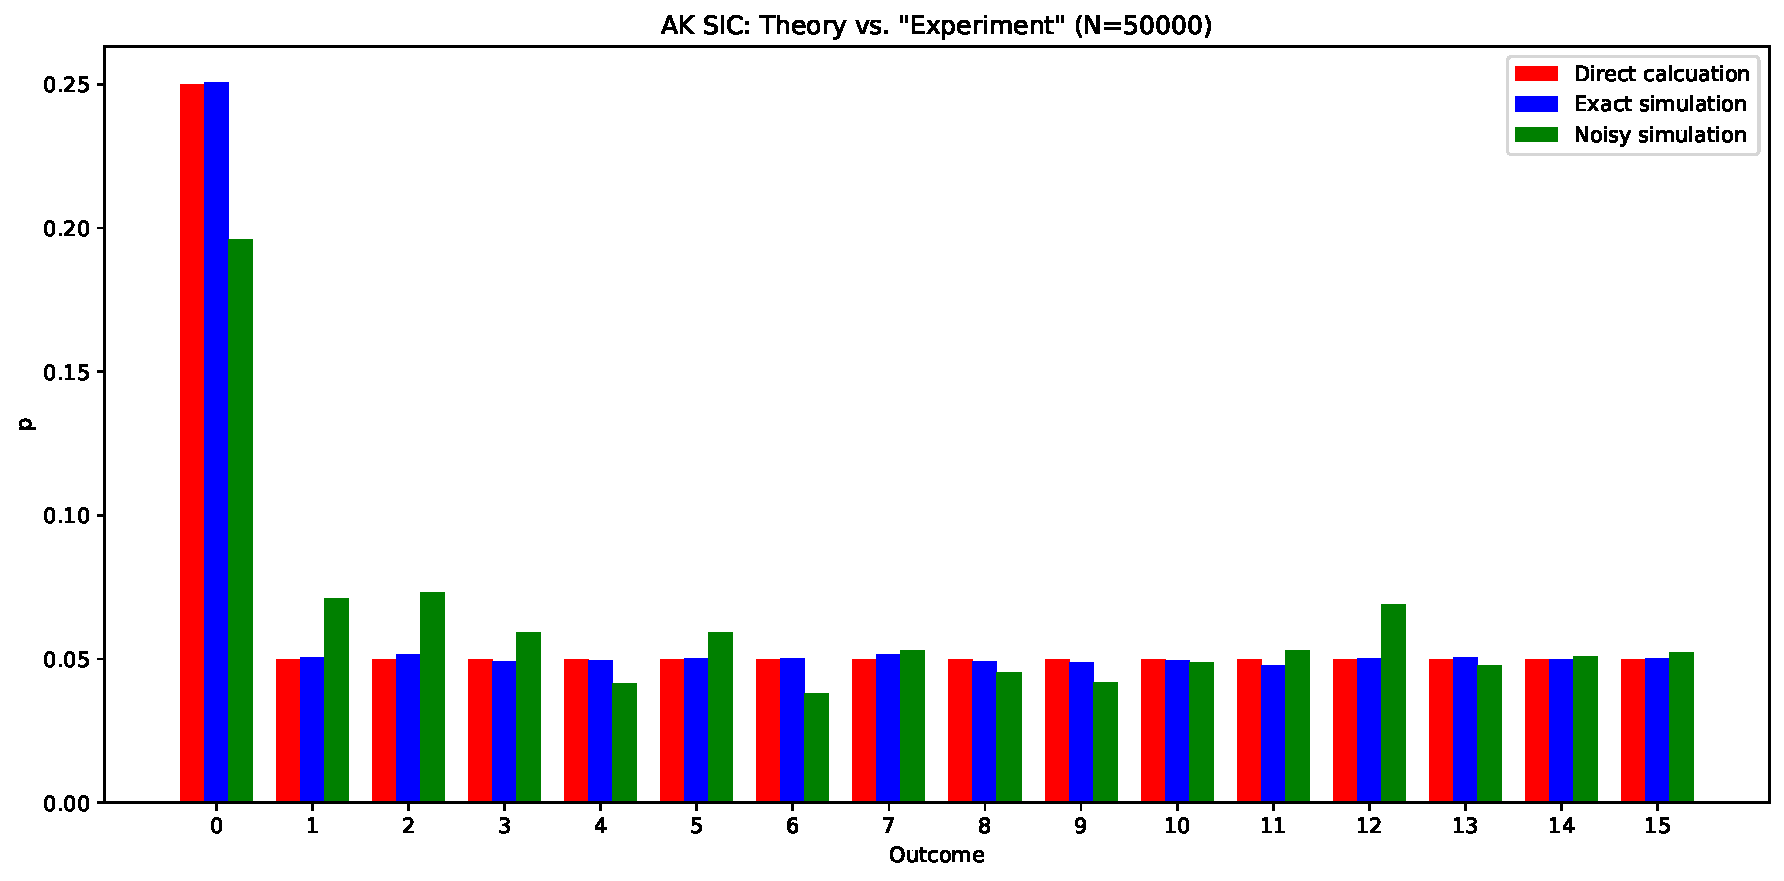
\includegraphics[scale=0.5]{img/ak_theory_vs_experiment}	
\end{center}


After conforming the circuit to the device's topology and optimizing it, the gate count by type for the full circuit, including the fiducial preparations, was
\begin{table}[h!]
\centering
\begin{tabular}{lr}
\toprule
\textbf{Gate Type} & \textbf{Count} \\
\midrule
PhasedXZGate    & 67 \\
CZPowGate       & 84 \\
PhasedXPowGate  & 99 \\
ZPowGate        & 10 \\
MeasurementGate & 1 \\
\bottomrule
\end{tabular}
\label{tab:circuit_gate_counts}
\end{table}


\noindent with a total of 153 moments. Below for 100,000 shots, we show on the left the exact conditional probability matrix 
\begin{align}
P(i,j)&= \frac{d\delta_{ij}+1}{d(d+1)}	
\end{align}
for a SIC outcome $i$ given a SIC state preparation $j$, in the middle the frequencies obtained from the noisy simulation, and on the right, the difference between the two. The Frobenius distance between them is $\lVert P_{\text{SIC}}-P\rVert \approx 0.3225$.
\begin{center}
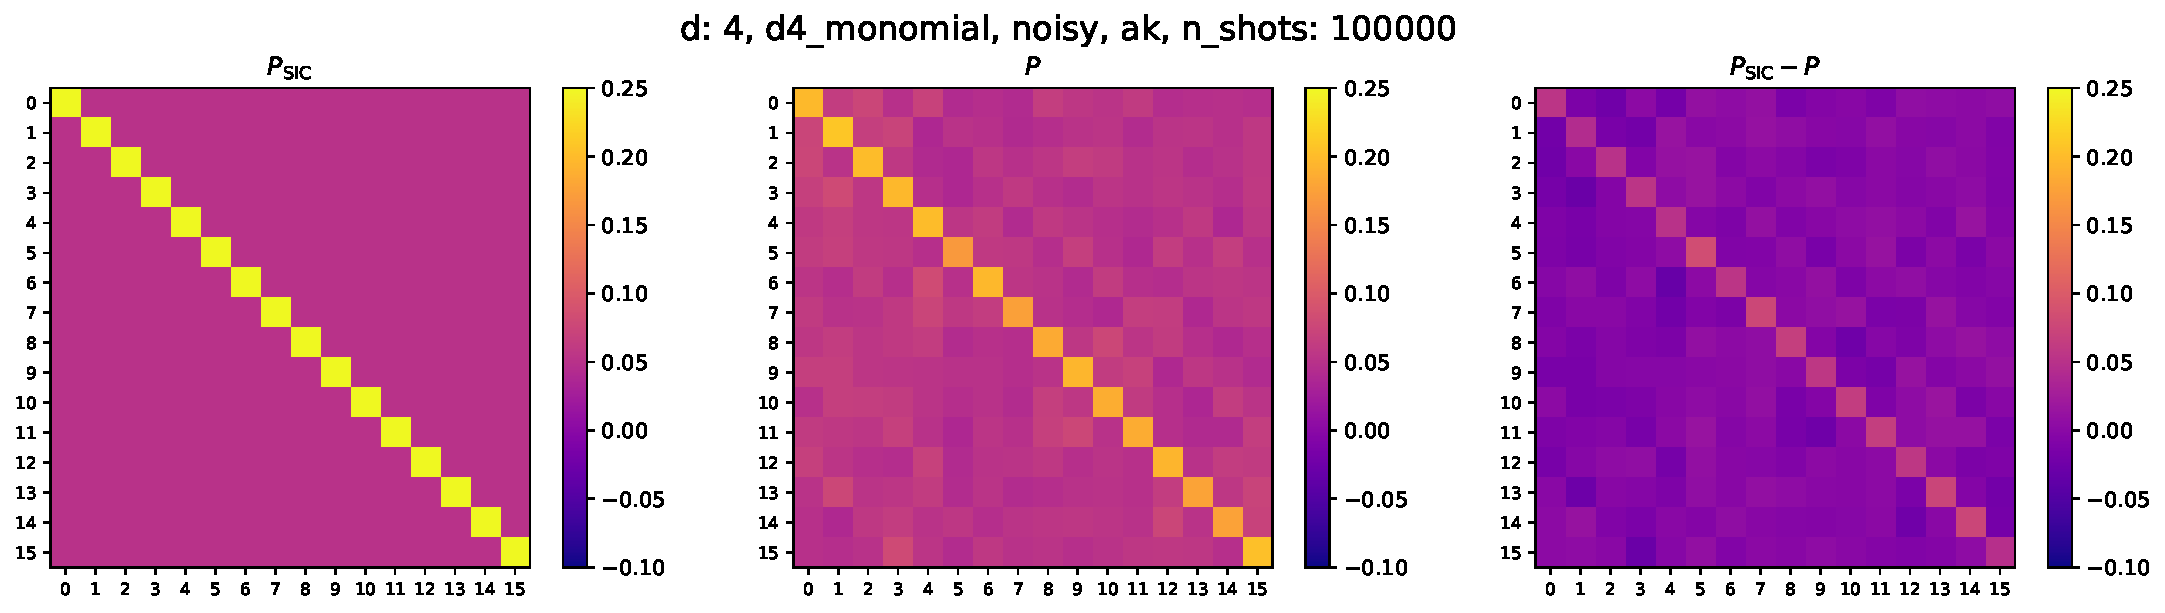
\includegraphics[scale=0.5]{img/P_d4_d4_monomial_noisy_ak_n100000}	
\end{center}


\section{A simplified WH-POVM procedure}
\label{simplifiedWH}
We now show that a WH-covariant POVM can be realized in a dramatically simpler way, analogous to the two-step measurement construction of \cite{Kalev_2012, PhysRevA.85.052115}, using a single ancilla system in the spirit of \cite{PhysRevA.86.062107}. Besides requiring a  smaller gate-count than the Arthurs-Kelly procedure, one benefit of our construction over the implementations cited in particular is that it cleanly separates out the preparation of the fiducial from the interaction which realizes the POVM. The downside is that the system is not projected into a state proportional to a POVM element at the end of the measurement, as in the Arthurs-Kelly procedure. Instead, at the end the qudits are left in a computational basis state.

To motivate the construction, we note that Eq. \!\ref{alt-gamma-expr} of Appendix \ref{alt-interpretation} shows that the initial state of the Arthurs-Kelly ancillas can be expressed
\begin{align}
\langle k, m|\gamma\rangle = 	d^{-3/2}\sum_{ab} \omega^{-am+bk}\tr(D_{a,b}^\dagger \Pi),
\end{align}
for desired fiducial $\Pi =|\phi\rangle\langle \phi|$. This implies that 

\begin{align}
|\gamma\rangle = (F\otimes F^\dagger )\frac{1}{\sqrt{d}}\sum_{ab}\tr(D_{a,b}^\dagger \Pi)|b,a\rangle.
\end{align}
Morever, we saw in Eq. \!\ref{ancilla-prep} that the initial state of the ancillas can be prepared from the fiducial by
\begin{align}
|\gamma\rangle=\left(\sum_j |j\rangle\langle j|\otimes Z^j	\right)\Big(I \otimes F^\dagger\Big)\Big(|\phi^*\rangle\otimes |\phi\rangle\Big).
\end{align}
Acting on the left of this expression with $F^\dagger \otimes F$, we conclude that \begin{align}
(F^\dagger \otimes I)\left(\sum_j |j\rangle\langle j|\otimes X^{-j}	\right)\Big(|\phi^*\rangle\otimes |\phi\rangle\Big)=\frac{1}{\sqrt{d}}\sum_{ab}\tr(D_{a,b}^\dagger \Pi)|b,a\rangle:
\end{align}
 $|\phi^*\rangle \otimes |\phi\rangle$ is transformed into $\frac{1}{\sqrt{d}}\sum_{ab}\tr(D_{a,b}^\dagger \Pi)|b,a\rangle$, whose components are proportional to the \emph{characteristic function} of the fiducial projector $\Pi$.  
 
 In fact, in preparing this state, we are effectively performing the WH-POVM itself. Re-aligning our conventions, let
 \begin{align}
 	\mathcal{D} &=(I\otimes F^\dagger)\left(\sum_j X^{-j}\otimes |j\rangle\langle j|\right)
 \end{align}
so that for an arbitrary state $|\psi\rangle$ and conjugate fiducial $|\phi^*\rangle$, 
\begin{align}
\Big(\langle a| \otimes \langle b|\Big)\mathcal{D}\Big(|\psi\rangle \otimes |\phi^*\rangle	\Big) &= 
\Big(\langle a| \otimes \langle b|\Big)(I\otimes F^\dagger)\left(\sum_j X^{-j}\otimes |j\rangle\langle j|\right)\Big(|\psi\rangle \otimes |\phi^*\rangle	\Big)\\
&=\sum_j \langle a|X^{-j}|\psi\rangle \langle b|F^\dagger |j\rangle\langle j|\phi^*\rangle\\
&=\frac{1}{\sqrt{d}}\sum_j \omega^{-bj}\langle\phi|j\rangle\langle j|X^{-a}|\psi\rangle \\
&=\frac{1}{\sqrt{d}}\sum_j \langle\phi|j\rangle\langle j|Z^{-b}X^{-a}|\psi\rangle \\
&=\frac{1}{\sqrt{d}}\langle \phi |D_{a,b}^\dagger |\psi\rangle.
\end{align}
It follows that the computational basis probabilities after performing $\mathcal{D}$ are 
\begin{align}
P(a,b)=\left|\frac{1}{\sqrt{d}}\langle \phi |D_{a,b}^\dagger |\psi\rangle\right|^2&=\frac{1}{d}\langle \psi |D_{a,b}|\phi\rangle\langle \phi |D_{a,b}^\dagger |\psi\rangle\\
&=\tr (E_{a,b}|\psi\rangle\langle \psi|),
\end{align}
where $E_{a,b}=\frac{1}{d}D_{a,b} \Pi D_{a,b}^\dagger$, and notice for simplicity we are conjugating in the opposite direction than usual. 

\subsection{A connection to ``magic state''}
Suppose we prepare $|\psi\rangle \otimes |\psi^*\rangle$. Recall for any pure state $\Pi=|\psi\rangle\langle \psi|$,  the \emph{stabilizer entropy} of order $\alpha$ may be defined as the R\'enyi entropy of  the probability distribution $P(a,b)$ we have just discussed,
\begin{align}
M_{\alpha}(|\phi\rangle)=\frac{1}{1-\alpha}\log \sum_{ab}P(a,b)^{\alpha} - \log d,
\end{align}
where $P(a,b) = \frac{1}{d}|\langle \psi|D_{a,b}^\dagger|\psi\rangle|^2$. 
The stabilizer entropy is a measure of the \emph{magic} of a quantum state: it achieves its minimum on so-called stabilizer states, and its maximum on SIC states \cite{cuffaro2024quantumstatesmaximalmagic}. Our construction provides a simple means of estimating it. Indeed, we note that
\begin{align}
\frac{1}{d}|\langle \psi |D_{a,b}^\dagger|\psi\rangle|^2 &= \frac{d\delta_{a,0}\delta_{b,0}+1}{d(d+1)}
\end{align}
if and only if  $\Pi = |\psi\rangle\langle \psi|$ is a SIC fiducial, so that we have efficient means of of testing fiducial preparations before implementing the full Arthurs-Kelly procedure. For further intuition about the matrix $\mathcal{D}$, consult appendix \ref{operatorD}. Finally, the gate counts for this simplified procedure (not counting the fiducial preparation) are:
\begin{table}[h!]
\centering
\begin{tabular}{lr}
\toprule
\textbf{Gate Type} & \textbf{Count} \\
\midrule
HPowGate    & 6 \\
CZPowGate   & 9 \\
SwapPowGate & 3 \\
\bottomrule
\end{tabular}
\label{tab:gate_counts_3}
\end{table}
\pagebreak

\subsection{Comparison}

We ran the simple WH-POVM circuit on the same noisy simulator, again performing a SIC-POVM on the $d=4$ SIC fiducial state.


\begin{center}
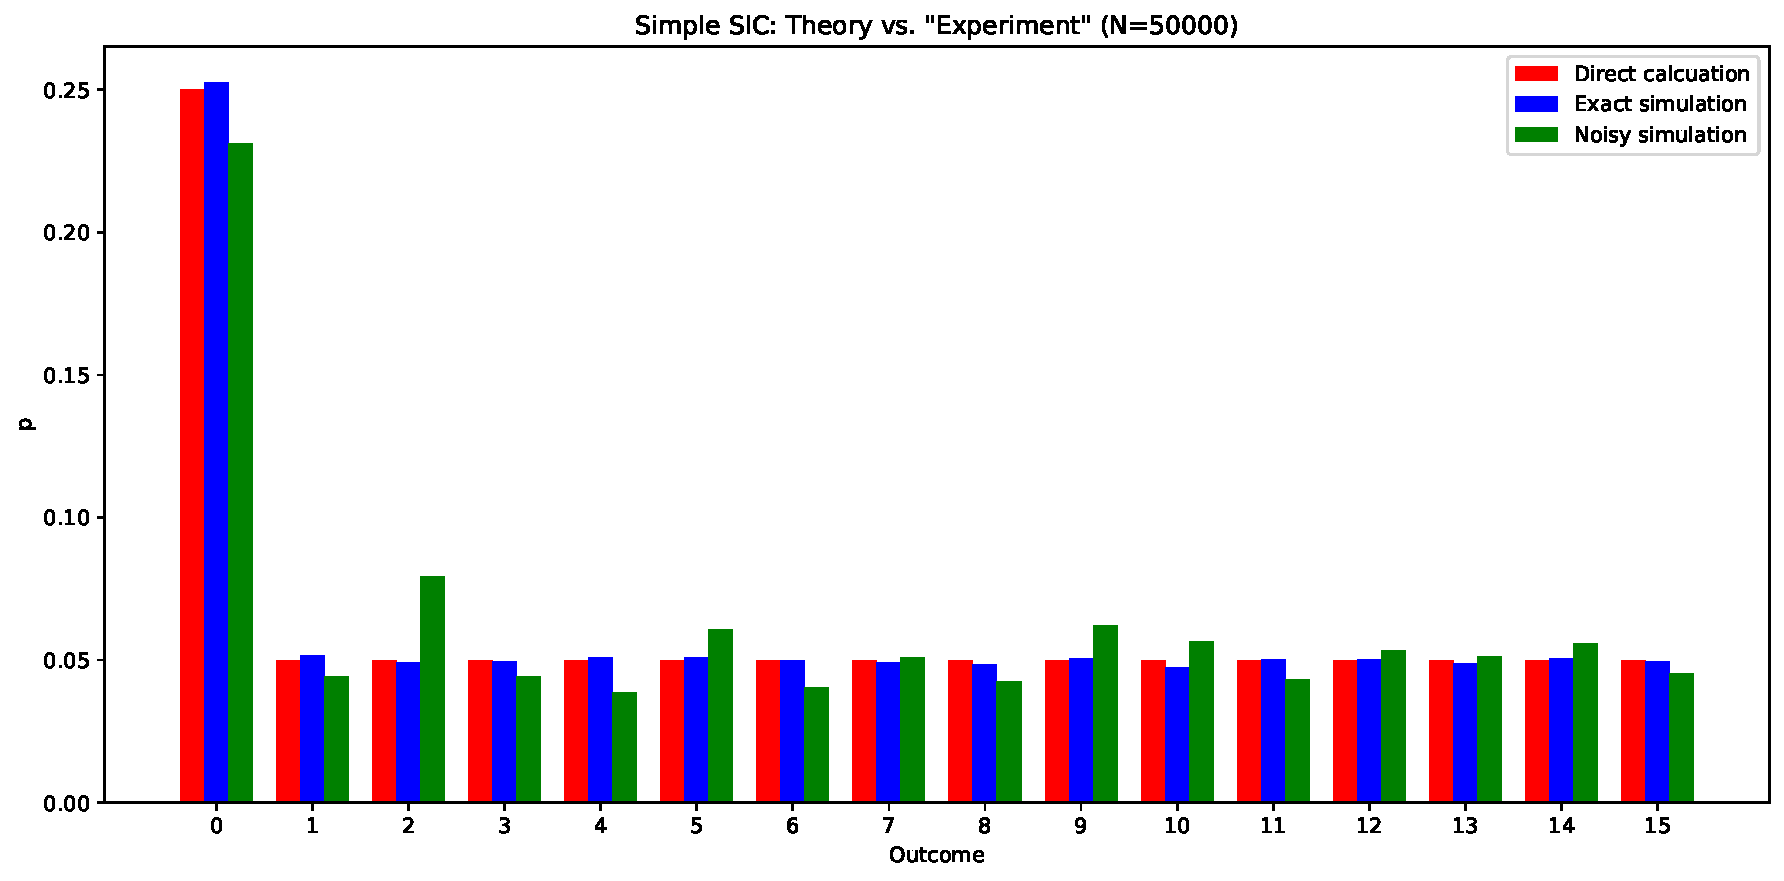
\includegraphics[scale=0.5]{img/simple_theory_vs_experiment}
\end{center}

The full gate counts including the fiducial preparation and after conforming the circuit to the device's topology and optimizing it are
\begin{table}[h!]
\centering
\begin{tabular}{lr}
\toprule
\textbf{Gate Type} & \textbf{Count} \\
\midrule
PhasedXPowGate  & 30 \\
CZPowGate       & 25 \\
PhasedXZGate    & 20 \\
MeasurementGate & 1 \\
\bottomrule
\end{tabular}
\label{tab:circuit_gate_counts_2}
\end{table}

\noindent with a total of 41 moments. For 100,000 shots, again we plot the frequencies for SIC outcomes given SIC states. Here $\lVert P_{\text{SIC}}-P\rVert|=0.2126$.
\begin{center}
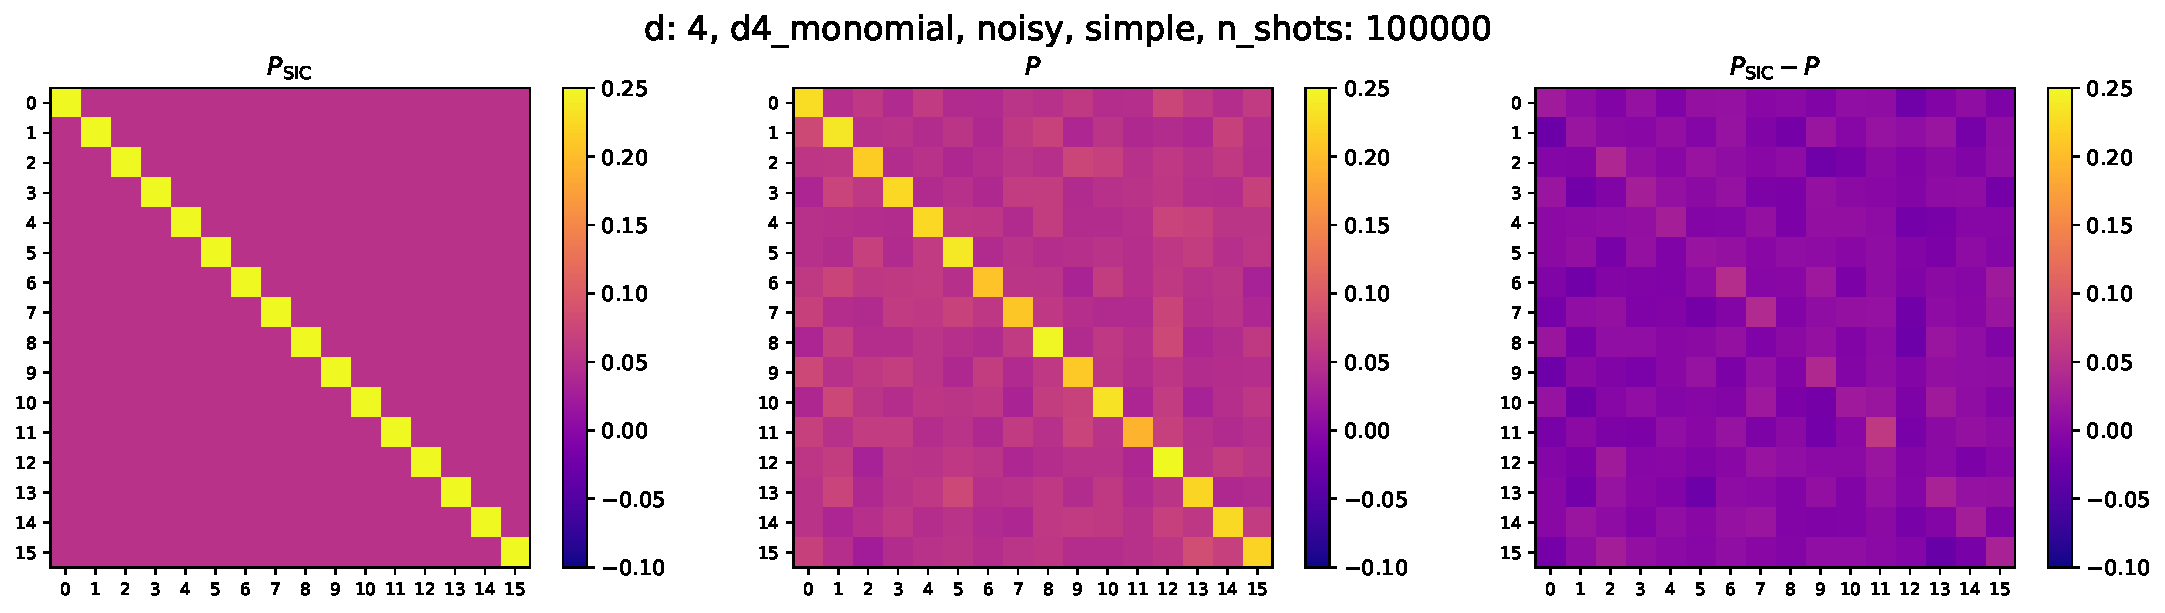
\includegraphics[scale=0.5]{img/P_d4_d4_monomial_noisy_simple_n100000}	
\end{center}

\section{The sky/ground scenario}

 
Fixing a Hilbert space dimension $d$, we call a \emph{reference device} a procedure which first performs an informationally complete measurement $\{R_i\}$, and then prepares one of a set of informationally complete states $\{\sigma_i\}$. Informational completeness means that the POVM elements (states, resp.) span the space of operators on $\mathcal{H}_d$: it follows that the reference measurement suffices to characterize an arbitrary state, and the reference states suffice to characterize an arbitrary measurement. 

In particular, by means of a IC reference device, the Born rule can  be re-expressed as a consistency condition across several experiments. Consider first preparing a quantum system according to $\rho$. We then send system into a reference device $\{R_i, \sigma_i\}$ that can be turned \emph{on} or \emph{off}. Afterwards, the system is sent into an arbitrary measurement $\{E_j\}$. 
\begin{center}
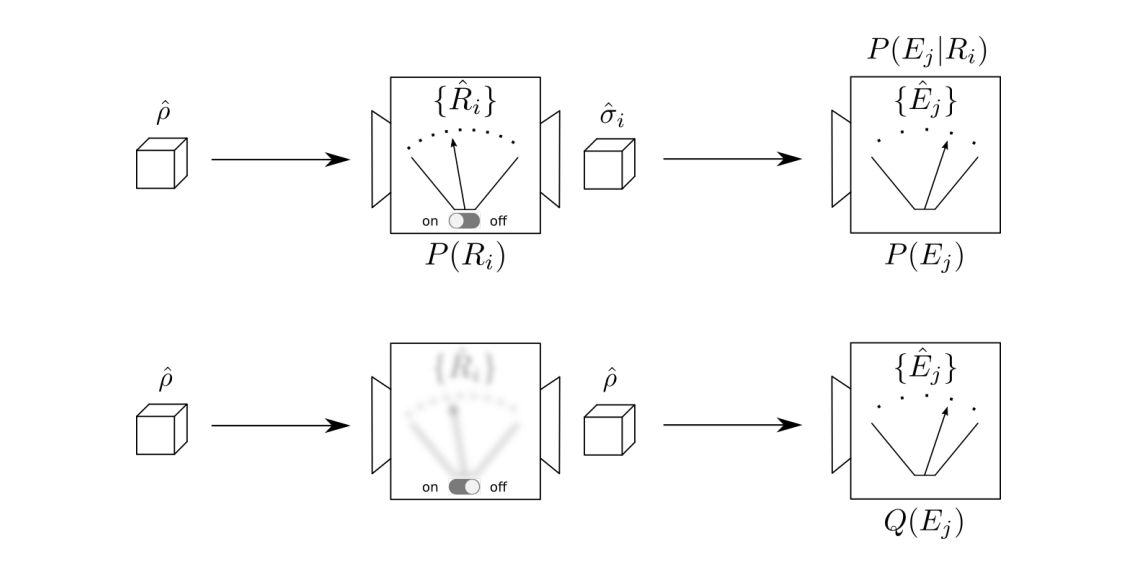
\includegraphics[scale=0.8]{img/sky_ground}	
\end{center}
In the first case, it is not hard to show that one's probability assignments ought to be related by the law of total probability,
\begin{align}
P(E_j)&=\sum_i P(E_j|R_i)P(R_i)	.
\end{align}
In the second case, when the reference device is turned off, by the Born rule we have
\begin{align}
Q(E_j)	&= \tr(E_j\rho).
\end{align}
But by informational-completeness, we ought to be able to rewrite this probability in terms of reference probabilities. Let us see how this can be done in a special case.

If the number of reference outcomes is $d^2$, the corresponding POVM elements must in fact form a linearly independent basis for the operator space. Let $|A)$ denote the vectorization of the matrix $A$, and recall that $\tr(B^\dagger A)= (B|A)$. Let $\B{R}_{ij}=(R_i|j)$ be the matrix whose rows are $(R_i|$ and and $\B{S}_{ij}=(i|S_j)$ be the matrix whose columns are $|\sigma_i)$. These are both $d^2 \times d^2$ matrices and by informational-completeness, $\B{R}$ and $\B{S}$  will in fact be invertible. Thus
\begin{align}
	Q(E_j)&=(E_j|\rho)=(E_j|\B{S}\B{S}^{-1}\B{R}^{-1}\B{R}|\rho)=(E_j|\B{S}(\B{RS})^{-1}\B{R}|\rho).
\end{align}
To interpret this expression, we note that $(E_j|\B{S}$ is the row vector of conditional probabilities $P(E_j|R_i)$, that $\B{R}|\rho)$ is the column vector of probabilities $P(R_i)$, and $\B{RS}=P$, the matrix of probabilities $P_{ij}=(R_i|\sigma_j)=P(R_i|R_j)$ for getting a reference outcome, given a reference state. Calling $\Phi \equiv P^{-1}$ the Born matrix, we've shown that
\begin{align}
Q(E_j)=\sum_{ik} P(E_j|R_i)\Phi_{ik}P(R_k).
\end{align}
In this way, the Born rule appears as a \emph{deformation} of the law of total probability by the operator $\Phi$, which is the inverse of the matrix $P$ which characterizes the reference device itself. In \cite{PhysRevResearch.2.013074}, the authors introduced as a measure of this deformation $||I-\Phi||$ with respect to any unitarily invariant norm, and proved that among all reference devices with $d^2$ outcomes,  $||I-\Phi||$ attains its minimum if and only if the reference measurement is a SIC and the reference states are proportional to its POVM elements, $\sigma_i = E_i/\tr(E_i)$. In this case, the expression for the Born rule simplifies to
\begin{align}
Q(E_j)=\sum_i P(E_j|R_i)\left[(d+1)P(R_i)-\frac{1}{d}\right]	.
\end{align}

To test this, let us consider the following set of conrete experiments:
\begin{enumerate}
\item Prepare each of the SIC states in turn, and then perform a SIC measurement. We can gather this data into a matrix of probabilities $P_{ij}=P(R_i|R_j)$.
\item Prepare each of the computational basis states $\{\Pi_i=|i\rangle\langle i|\}$, and then perform a SIC measurement. We can gather the probabilities into a matrix $p_{ij} = P(R_j|\Pi_i)$.
\item Prepare each of the SIC states, and perform a computational basis measurement, yielding a matrix of probabilities $C_{ij}=P(\Pi_i|R_j)$.
\item Prepare each of the computational basis states, and perform a computational basis measurement, yielding probabilities $q_{ij}=P(\Pi_i|\Pi_j)$.
\end{enumerate}
Letting $\Phi=P^{-1}$, the Born rule then demands the following consistency condition,
\begin{align}
q = C\Phi p.	
\end{align}
In order to measure the extent to which our matrices violate this criterion, we could consider several metrics. In order to evaluate the implementation of the SIC itself, we could consider $\lVert P-P_{\text{SIC}}\rVert$, where $P_{\text{SIC}}$ are the exact probabilities, using the Frobenius norm. Alternatively, we could consider $\lVert \Phi -\Phi_{\text{SIC}}\rVert$, or even $\lVert I - \Phi \rVert$, since the latter is known to be minimized over all reference devices for SIC's alone. 
\begin{center}
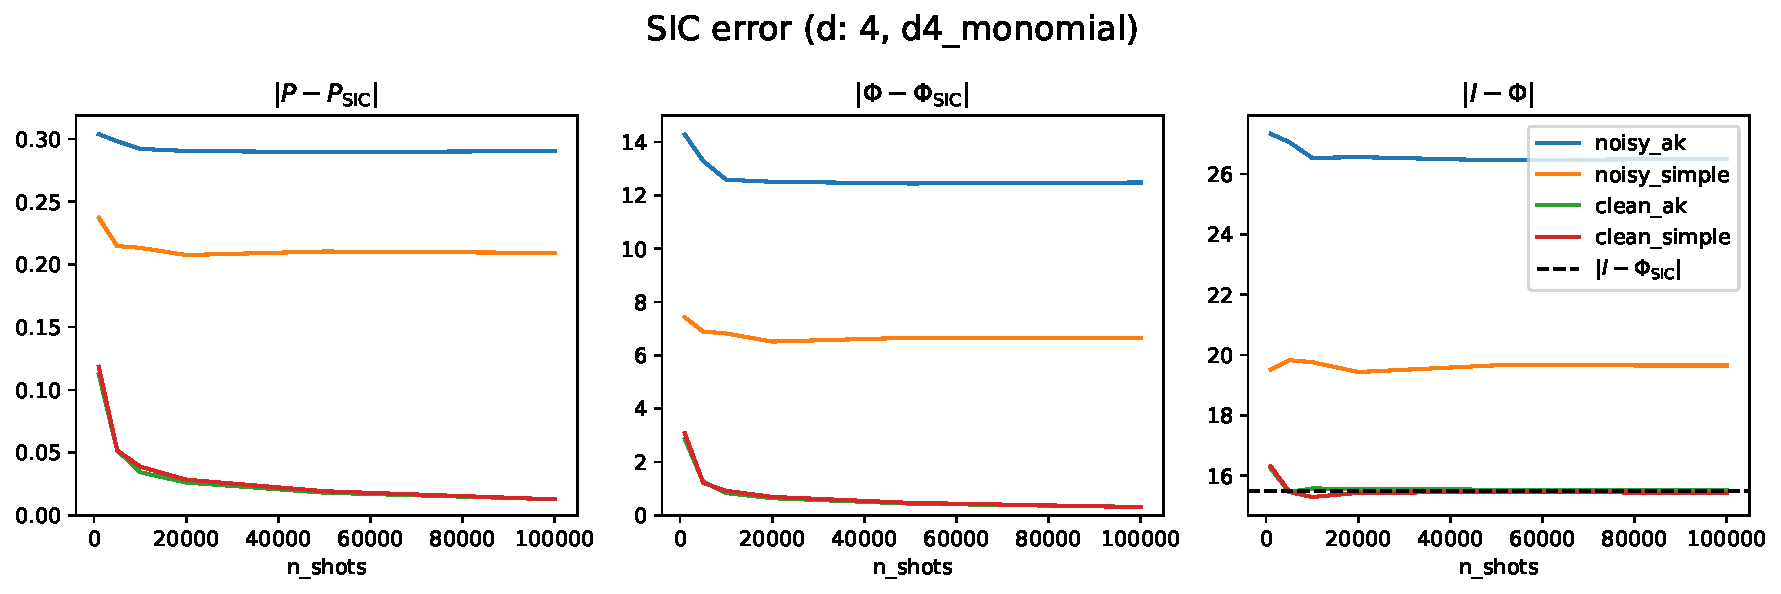
\includegraphics[scale=0.55]{img/sic_metrics_d4_d4_monomial}	
\end{center}
Above we plot these three metrics as functions of the number of repetitions of the experiment. In blue, we plot the error for the Arthurs-Kelly implementation of a SIC in the presence of simulated noise. In orange, the same for the simpler WH-POVM implementation. The error for simulations without noise are in green and red. Clearly, in the latter case, as the number of samples increases, the error approaches zero. For the noisy simulations, however, the error plateaus, although the simpler algorithm decisively outperforms the full Arthurs-Kelly procedure.

We could also consider the metrics which account for the whole Born rule itself. First, we consider $\lVert I - q\rVert$. Recall that $q_{ij}$ is the probability with which we obtain a computational basis outcome $i$, given that we prepared computational basis $j$. Clearly, this ought to be the $d\times d$ identity matrix. We see, however, that in the presence of noise, this is not true. Next, we consider $\lVert q-C\Phi p\rVert$, which quantifies the error in the probability-based Born rule itself. Again, in the presence of noise, after decreasing initially, the error plateaus.
\begin{center}
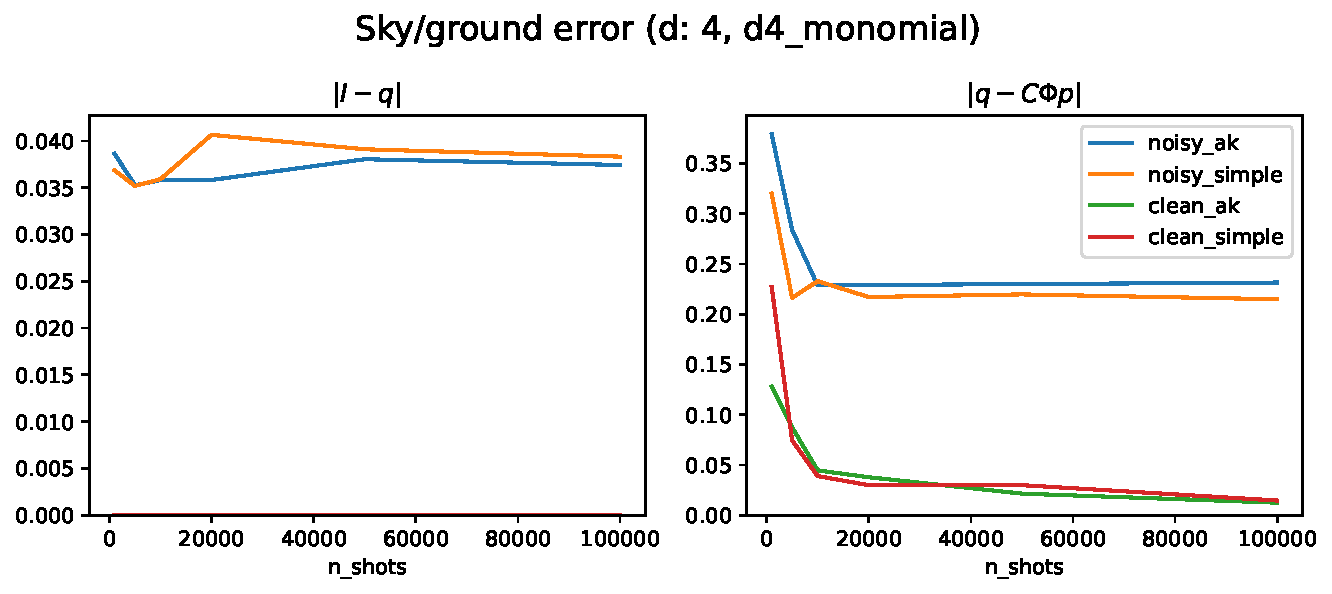
\includegraphics[scale=0.55]{img/sg_metrics_d4_d4_monomial}	
\end{center}
To better visualize this, we plot the elements of these matrices after 100,000 shots.
\begin{center}
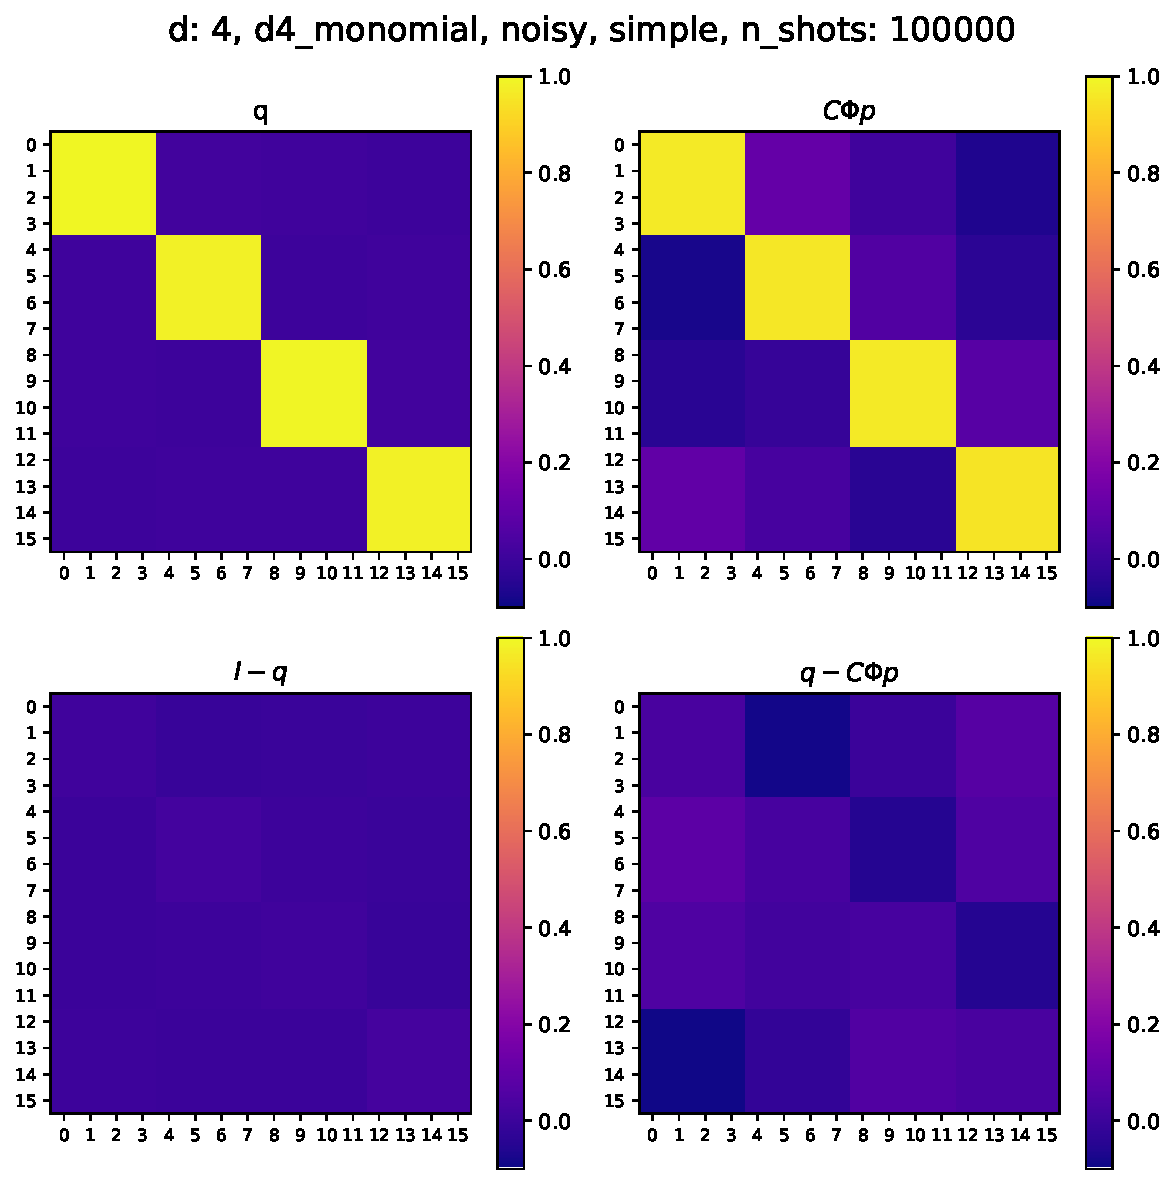
\includegraphics[scale=0.4]{img/q_d4_d4_monomial_noisy_simple_n100000}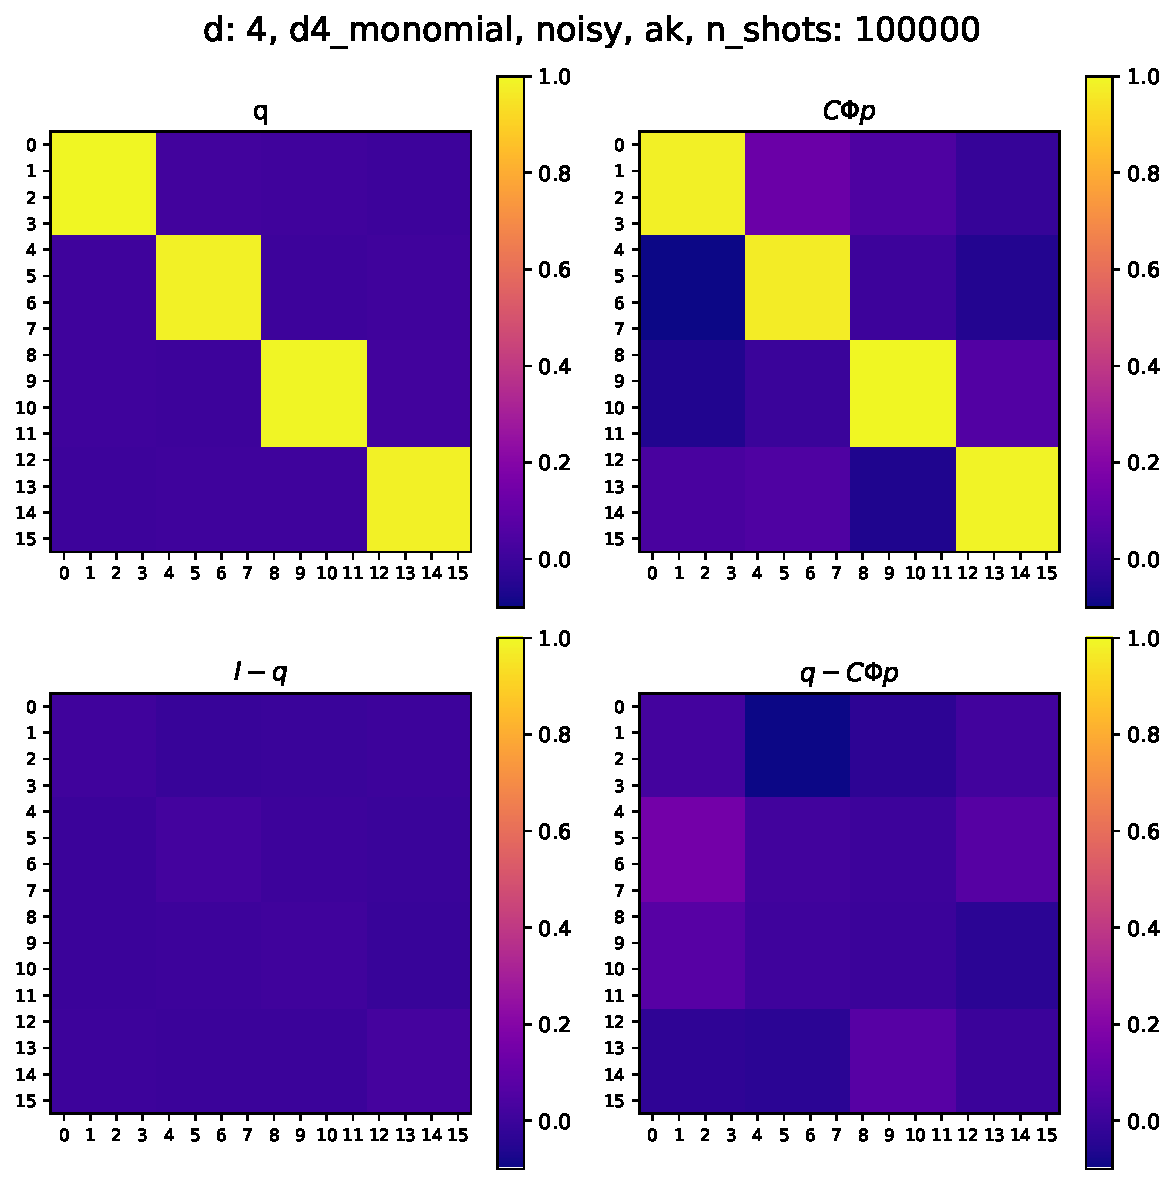
\includegraphics[scale=0.4]{img/q_d4_d4_monomial_noisy_ak_n100000}	
\end{center}
On the left is the results for the simple WH-POVM implementation, and on the right the same for the Arthurs-Kelly. For both, $\lVert I - q\rVert \approx 0.056$, which shows that even in the simplest scenario of a computational basis preparation, and a computational basis measurement, there is considerable noise. Meanwhile, for the former, $\lVert q - C \Phi p\rVert \approx 0.2271$, and for the latter, $\lVert q - C \Phi p\rVert \approx 0.2618$. 

\section{WH-POVM's for any $d=2^n$}

In order to perform WH-POVM's in any dimension $d=2^n$ with arbitrary fiducial states, it is useful to consider a general state preparation ansatz which, given a state vector $|\psi\rangle$, generates a circuit of single qubit rotations and \T{CNOT}'s which prepares it. In particular, we would ideally use an ansatz for which it is as easy to prepare the complex conjugate of a state as the state itself. An example is provided by \cite{1629135}, which realizes a state by a sequence of block diagonal unitaries whose blocks are $Y$ and $Z$ rotations. These ``uniformly controlled rotations'' can be implemented by the scheme provided by \cite{PhysRevLett.93.130502} which exploits the binary reflected Gray code, as explained in Appendix \ref{ansatz_explanation}. Using known numerical solutions for SIC fiducials, we may then compare SIC sky/ground scenarios in $d=2,4,8$ using this scheme.

\subsection{$d=2$}
\begin{center}
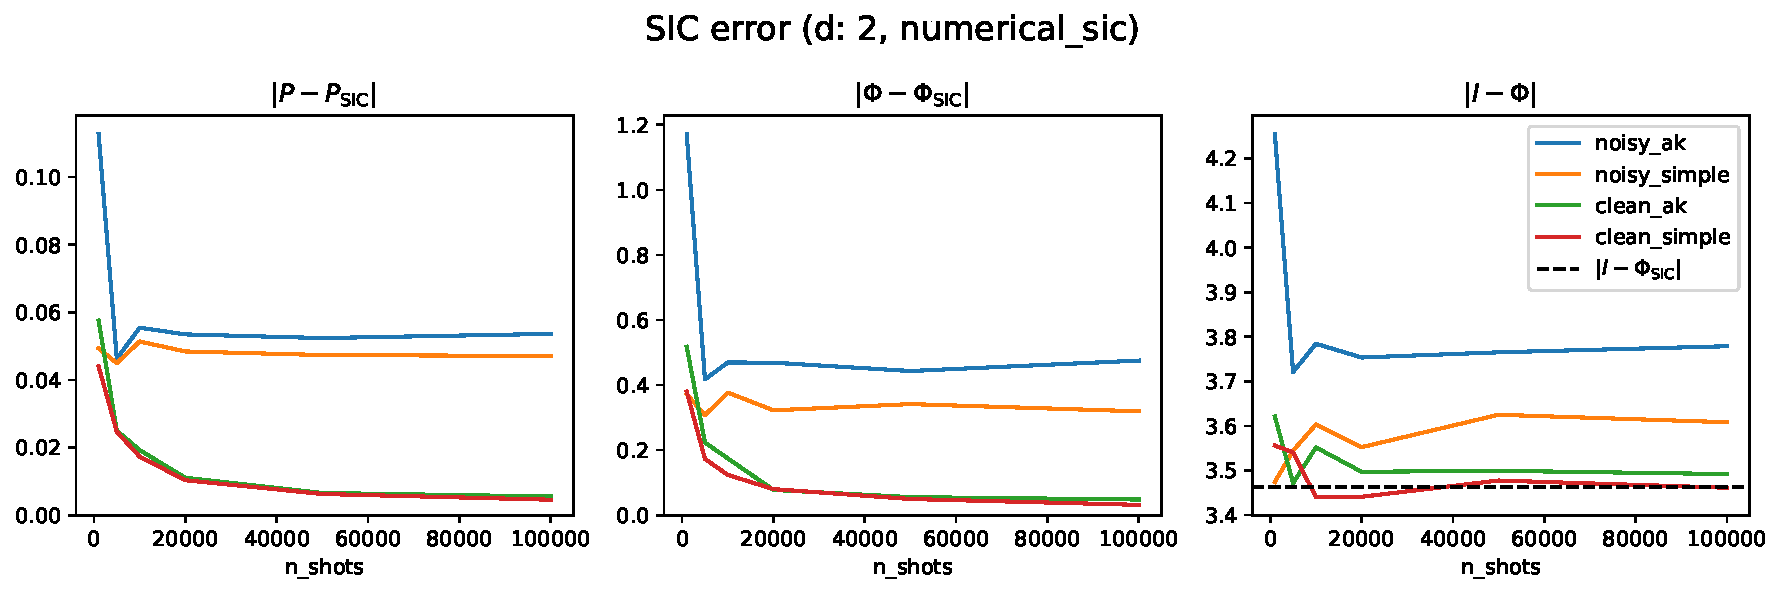
\includegraphics[scale=0.5]{img/sic_metrics_d2_numerical_sic}	

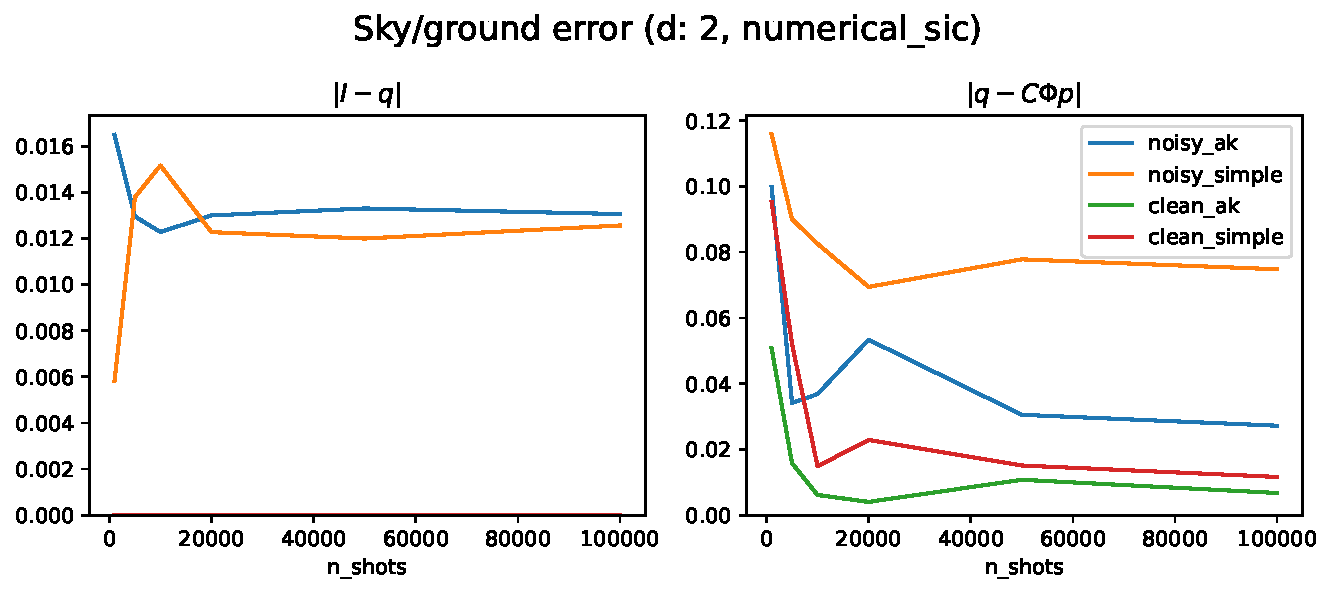
\includegraphics[scale=0.5]{img/sg_metrics_d2_numerical_sic}	

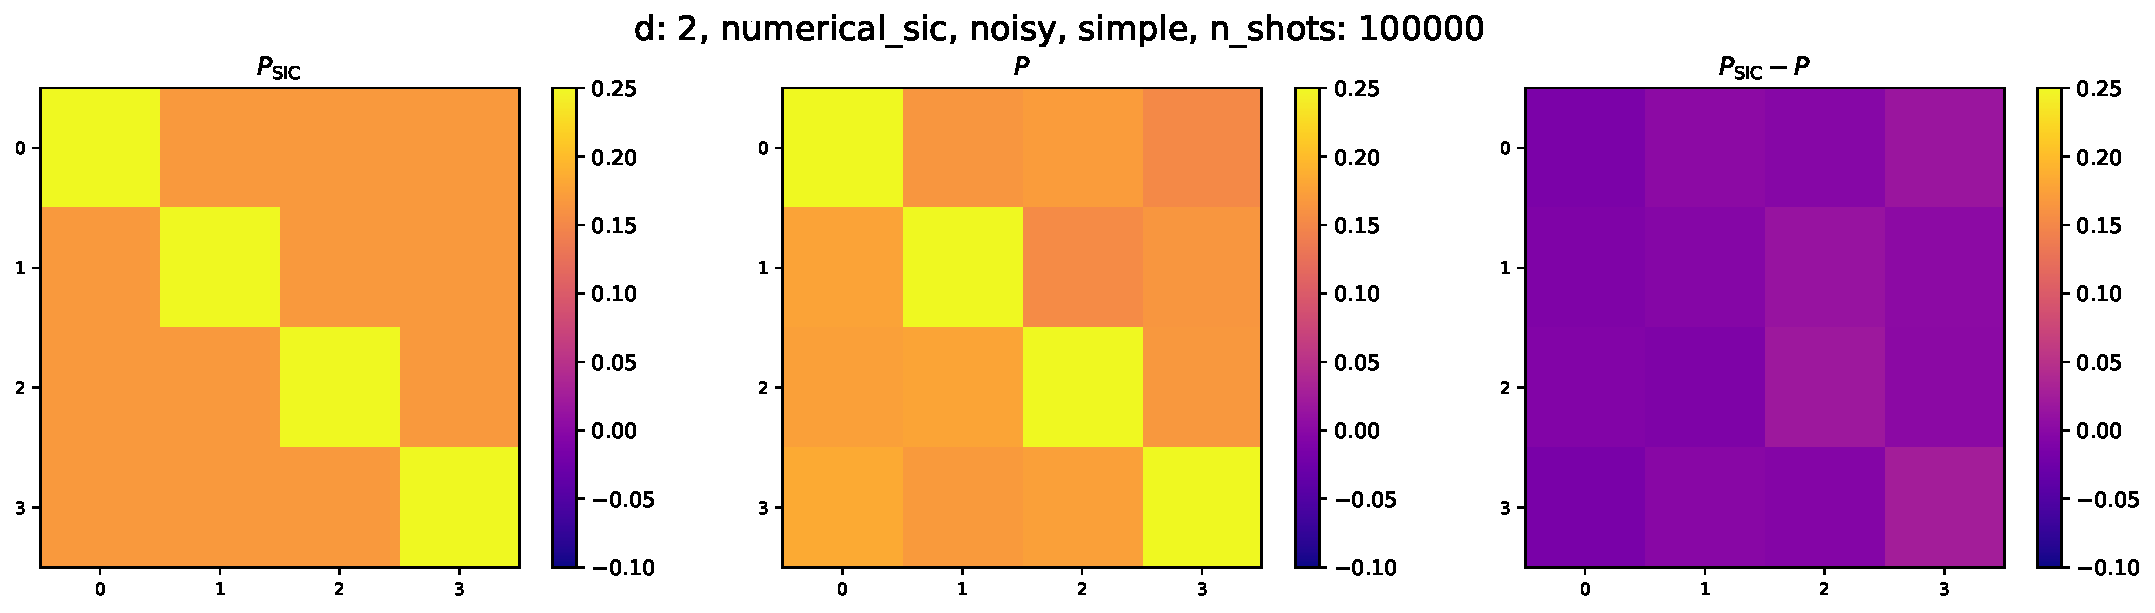
\includegraphics[scale=0.4]{img/P_d2_numerical_sic_noisy_simple_n100000}

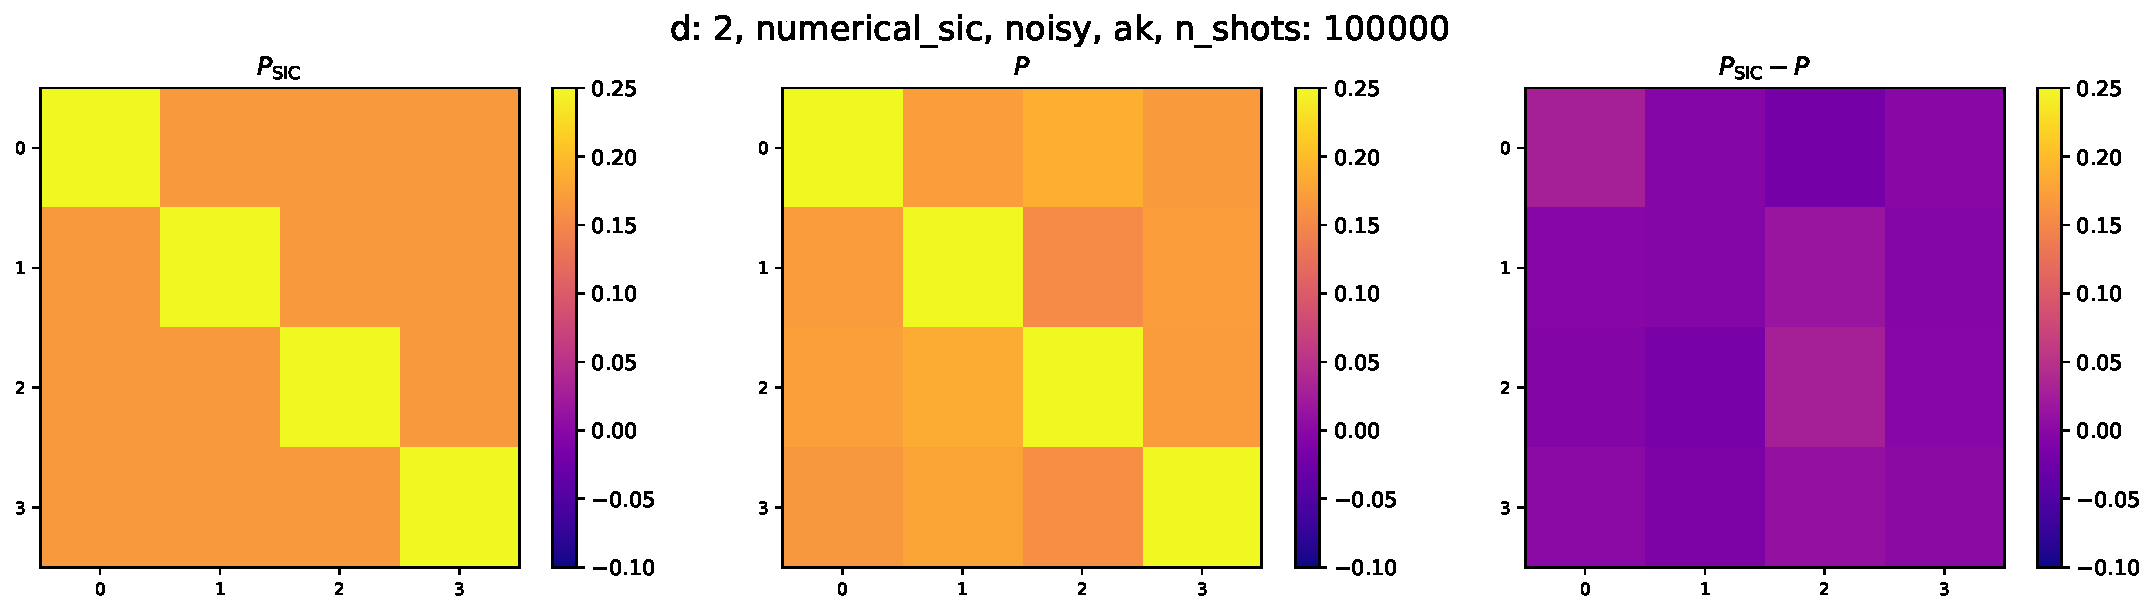
\includegraphics[scale=0.4]{img/P_d2_numerical_sic_noisy_ak_n100000}

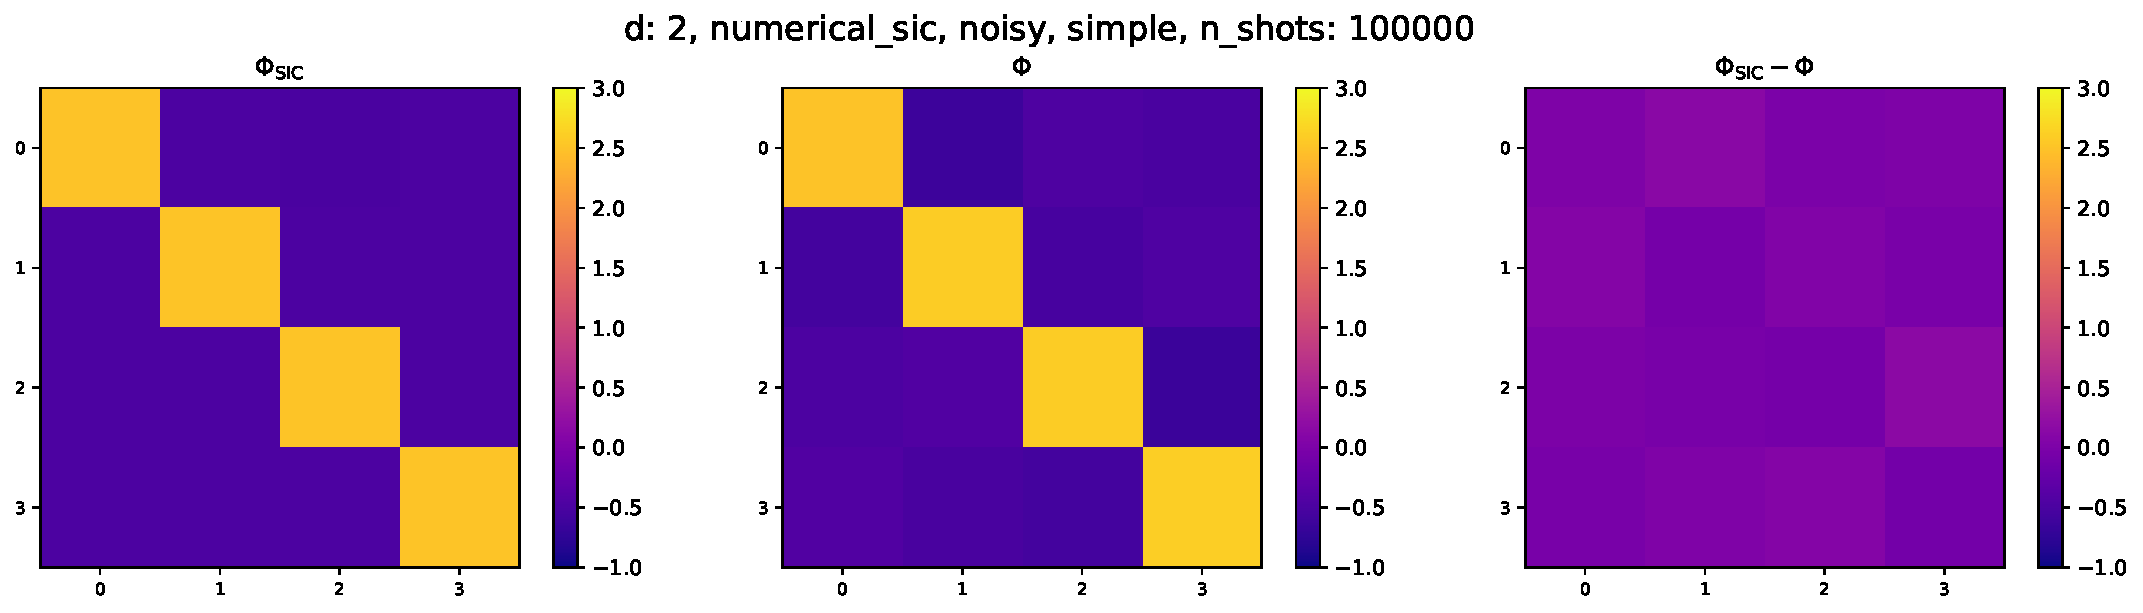
\includegraphics[scale=0.4]{img/Phi_d2_numerical_sic_noisy_simple_n100000}

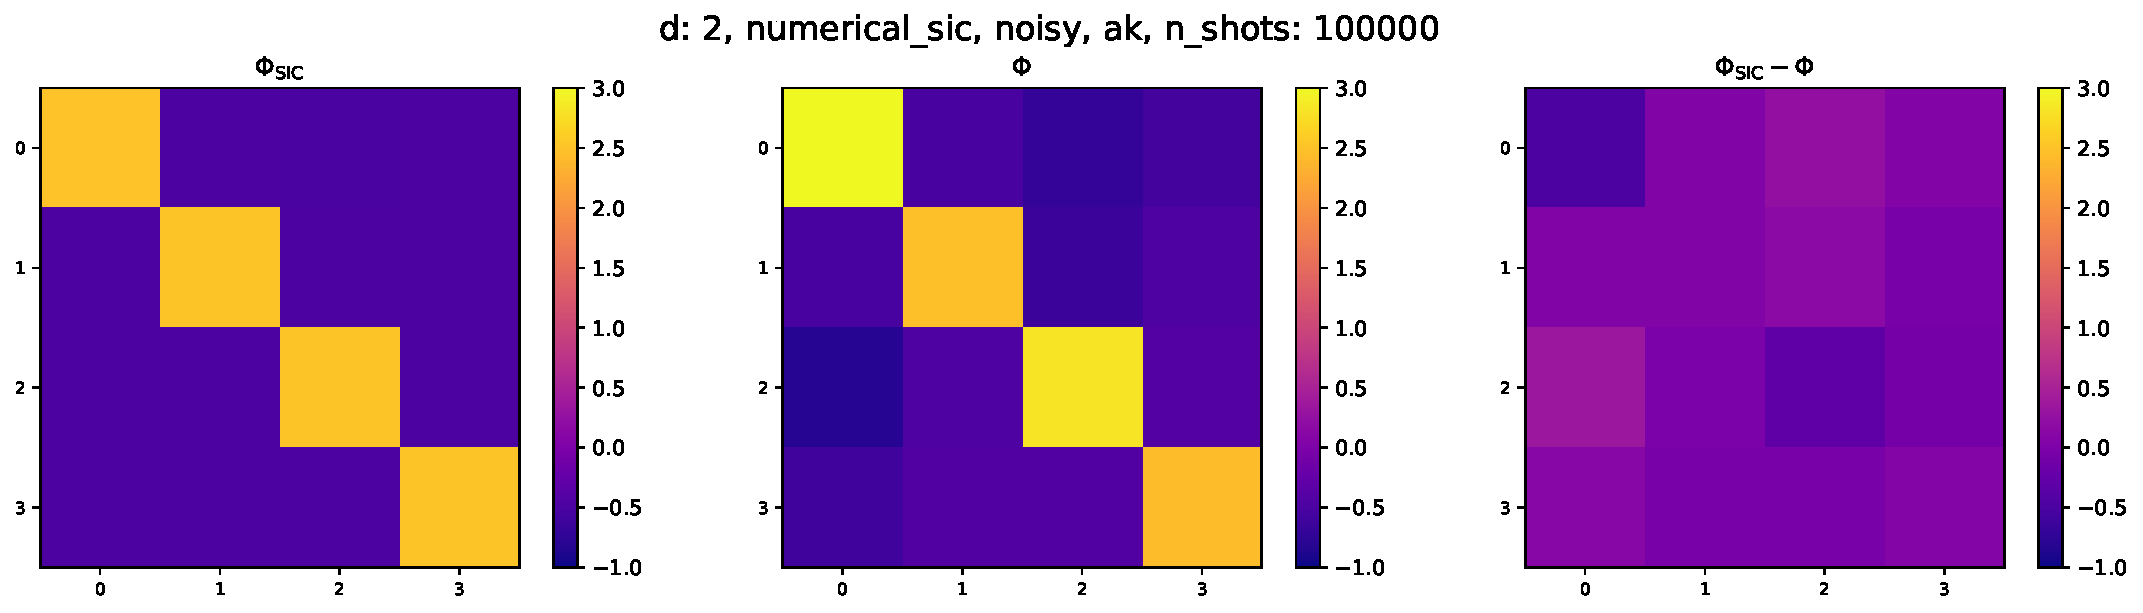
\includegraphics[scale=0.4]{img/Phi_d2_numerical_sic_noisy_ak_n100000}

\end{center}

\subsection{$d=4$}

\begin{center}
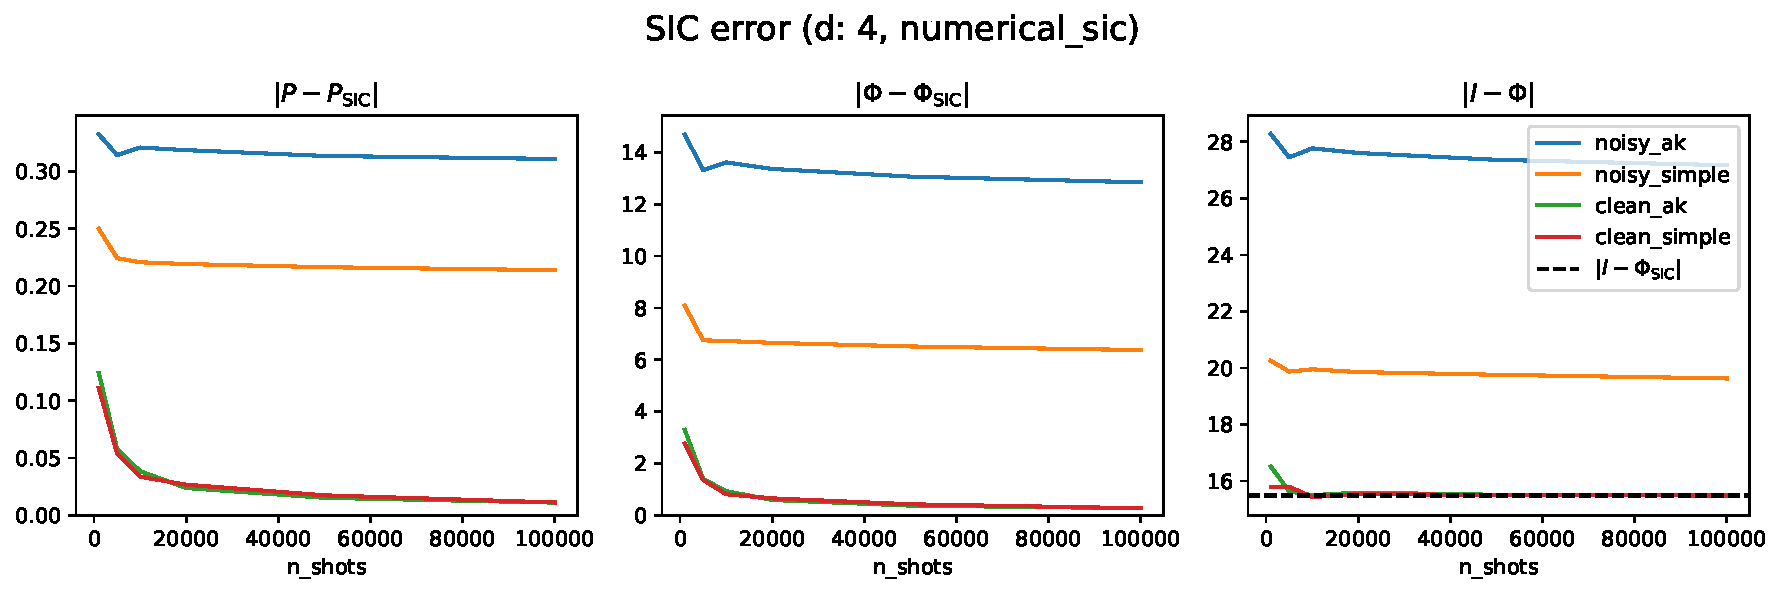
\includegraphics[scale=0.5]{img/sic_metrics_d4_numerical_sic}	

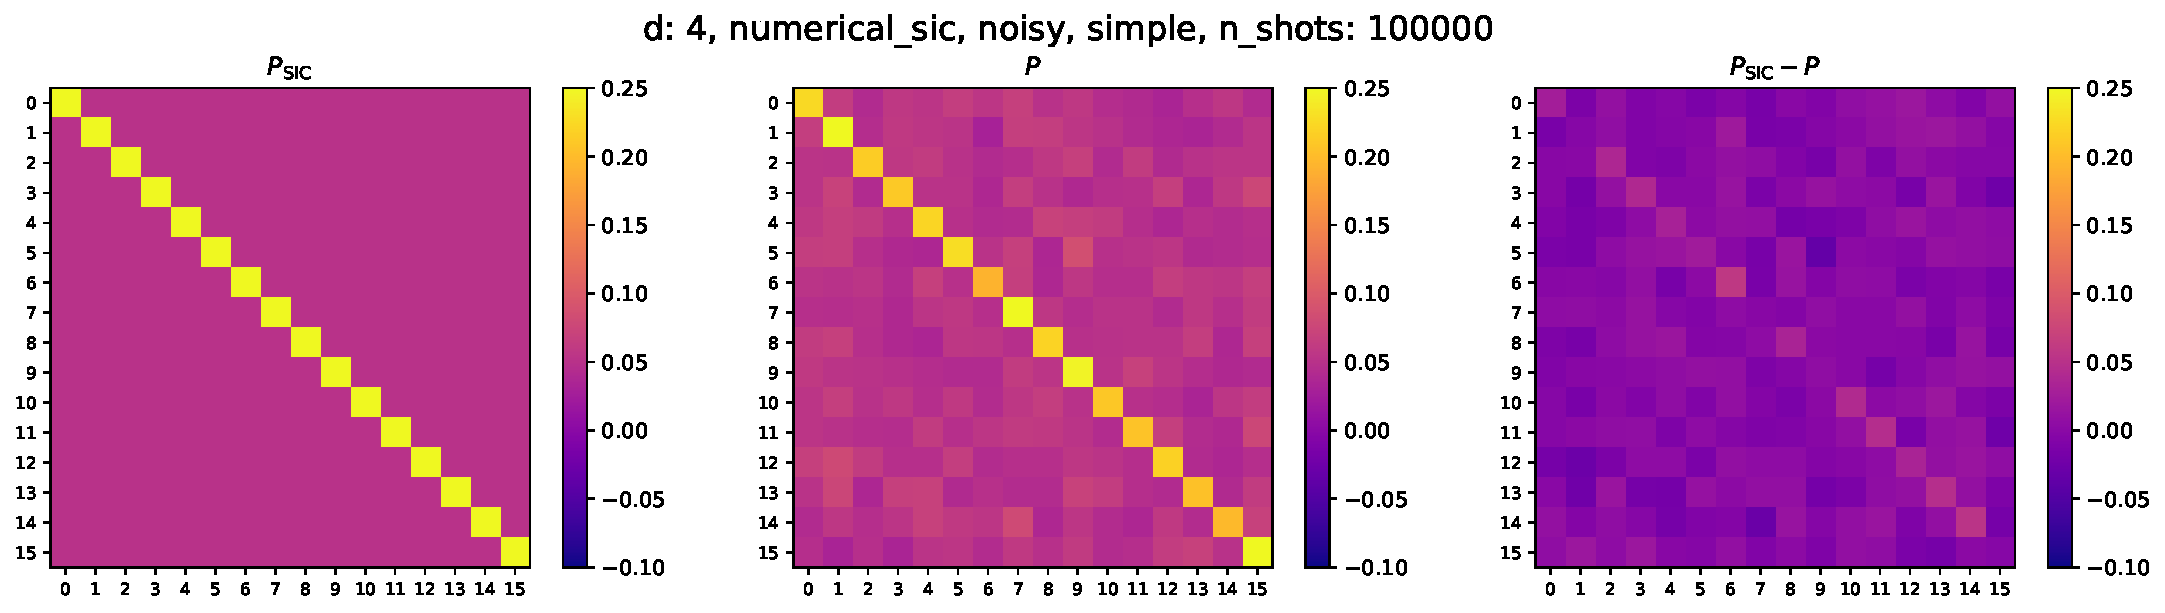
\includegraphics[scale=0.4]{img/P_d4_numerical_sic_noisy_simple_n100000}

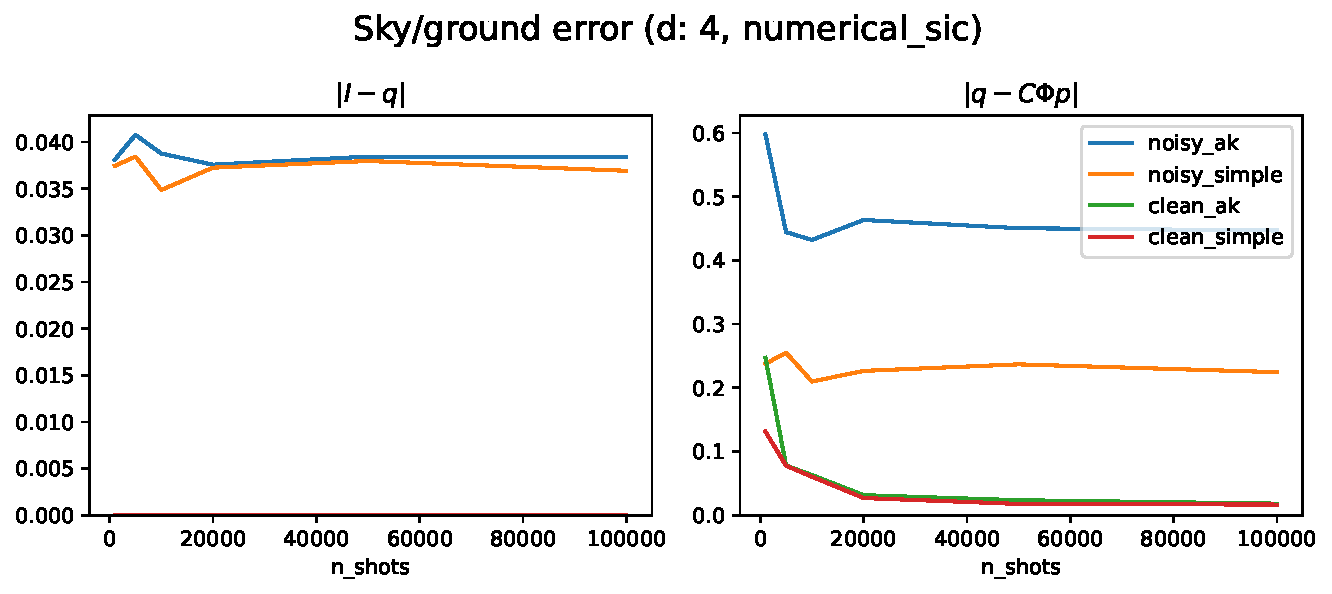
\includegraphics[scale=0.5]{img/sg_metrics_d4_numerical_sic}	

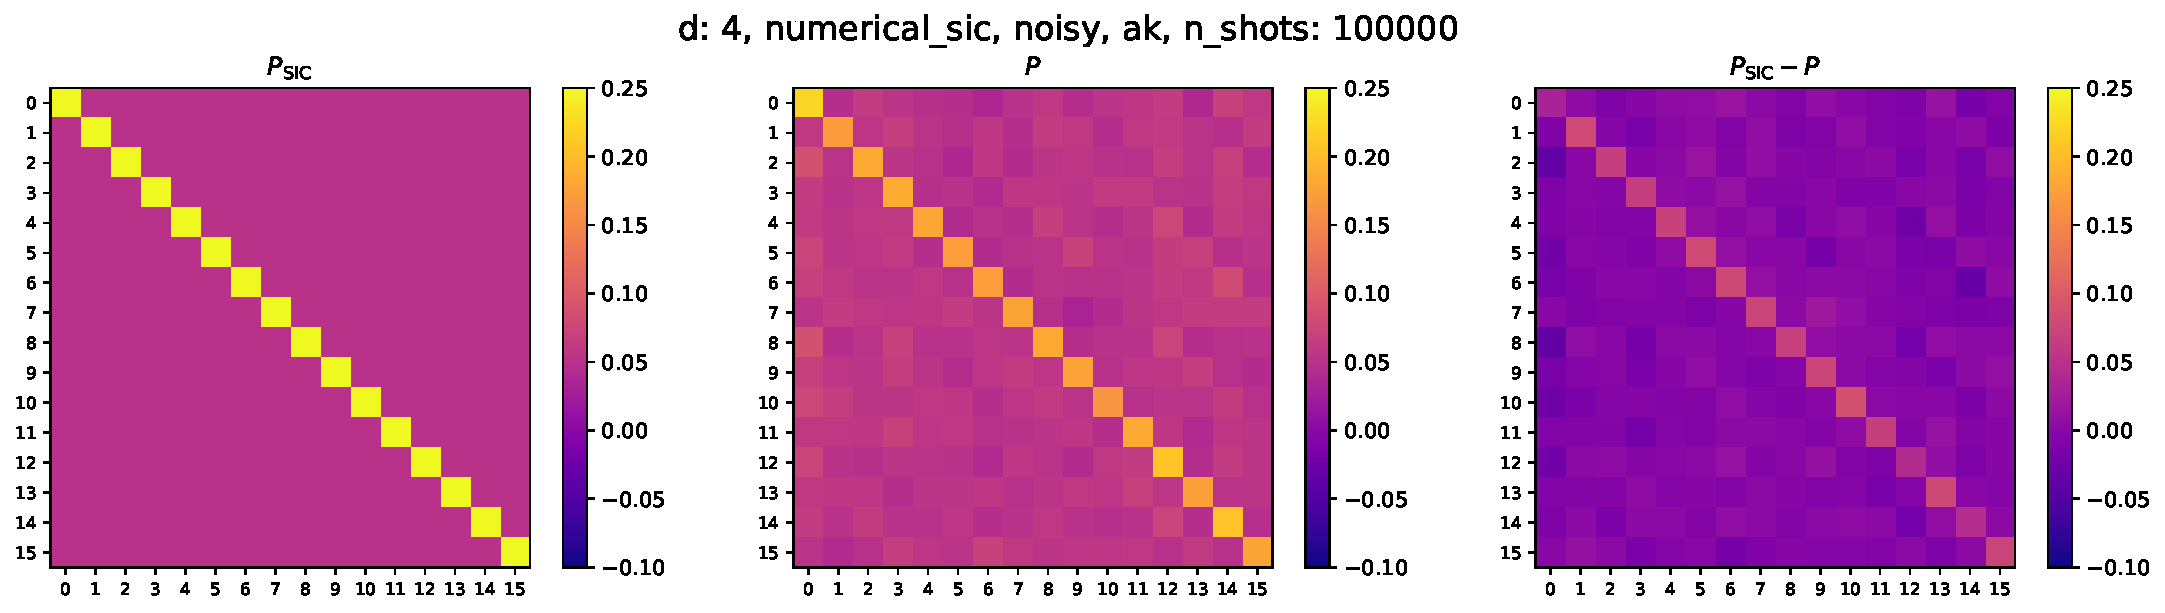
\includegraphics[scale=0.4]{img/P_d4_numerical_sic_noisy_ak_n100000}

\end{center}

\subsection{$d=8$}

\begin{center}
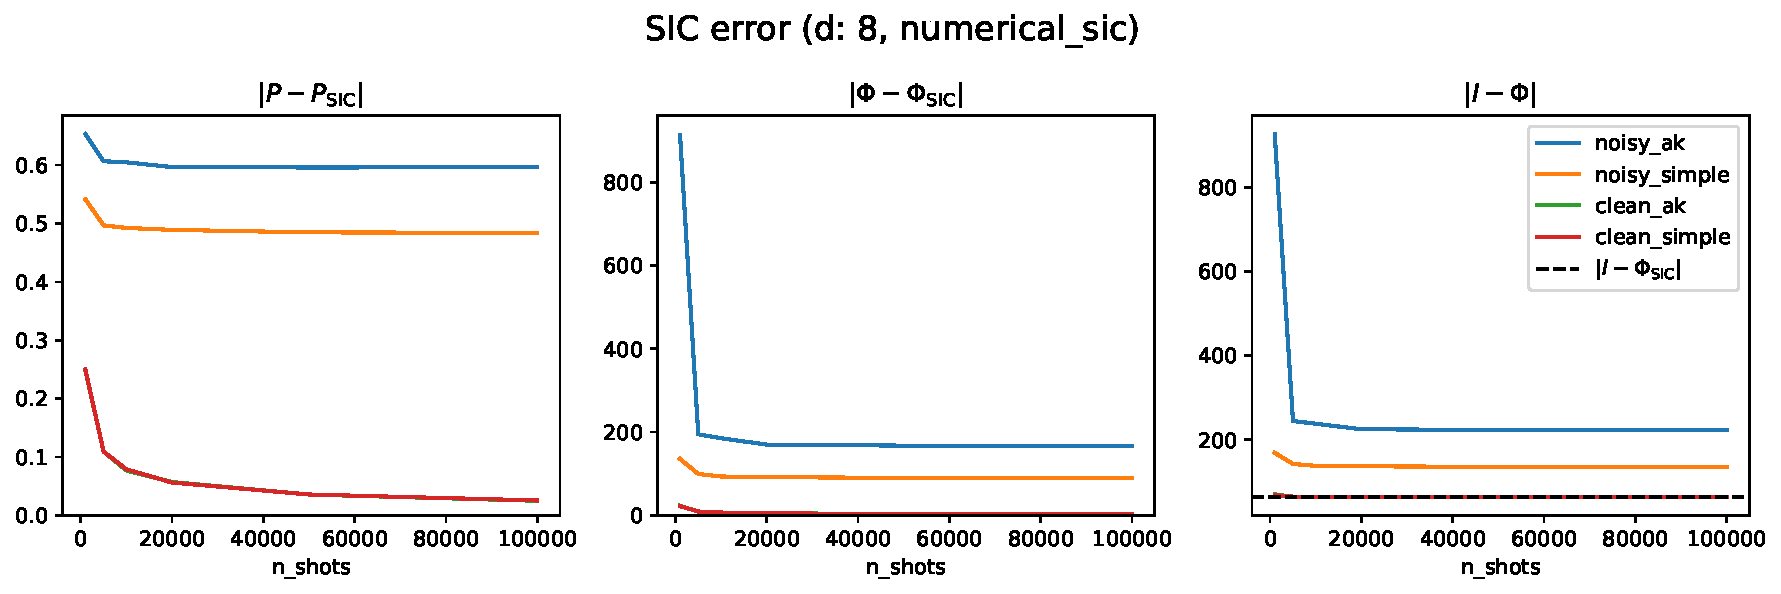
\includegraphics[scale=0.5]{img/sic_metrics_d8_numerical_sic}	

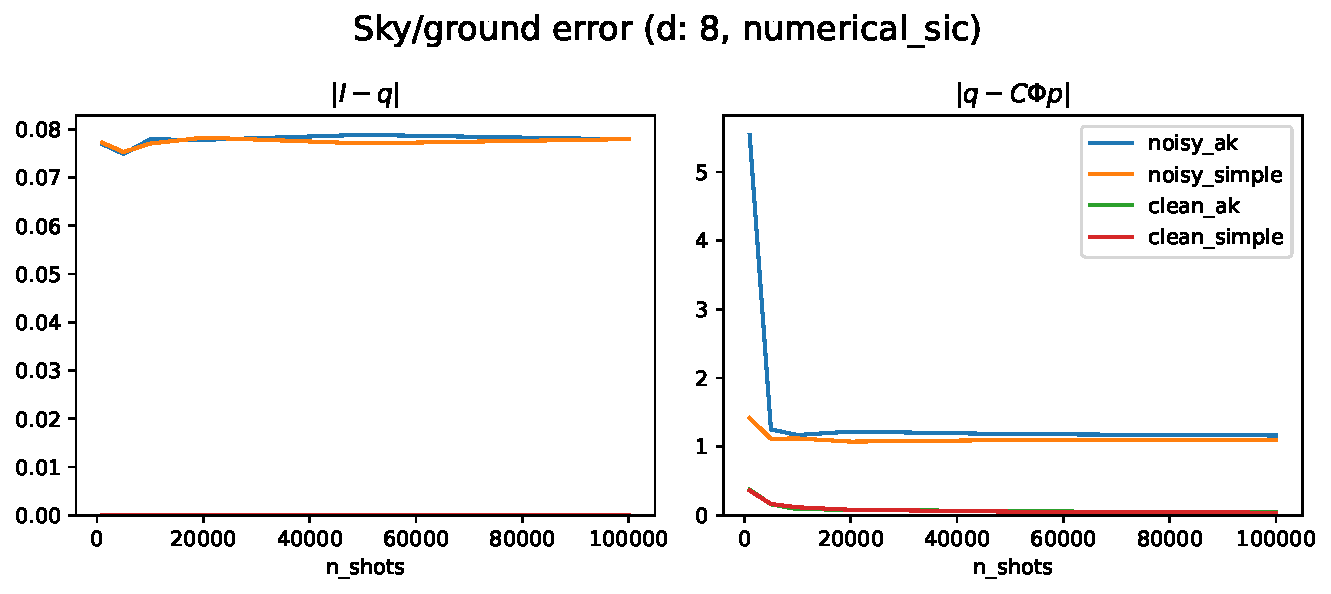
\includegraphics[scale=0.5]{img/sg_metrics_d8_numerical_sic}	

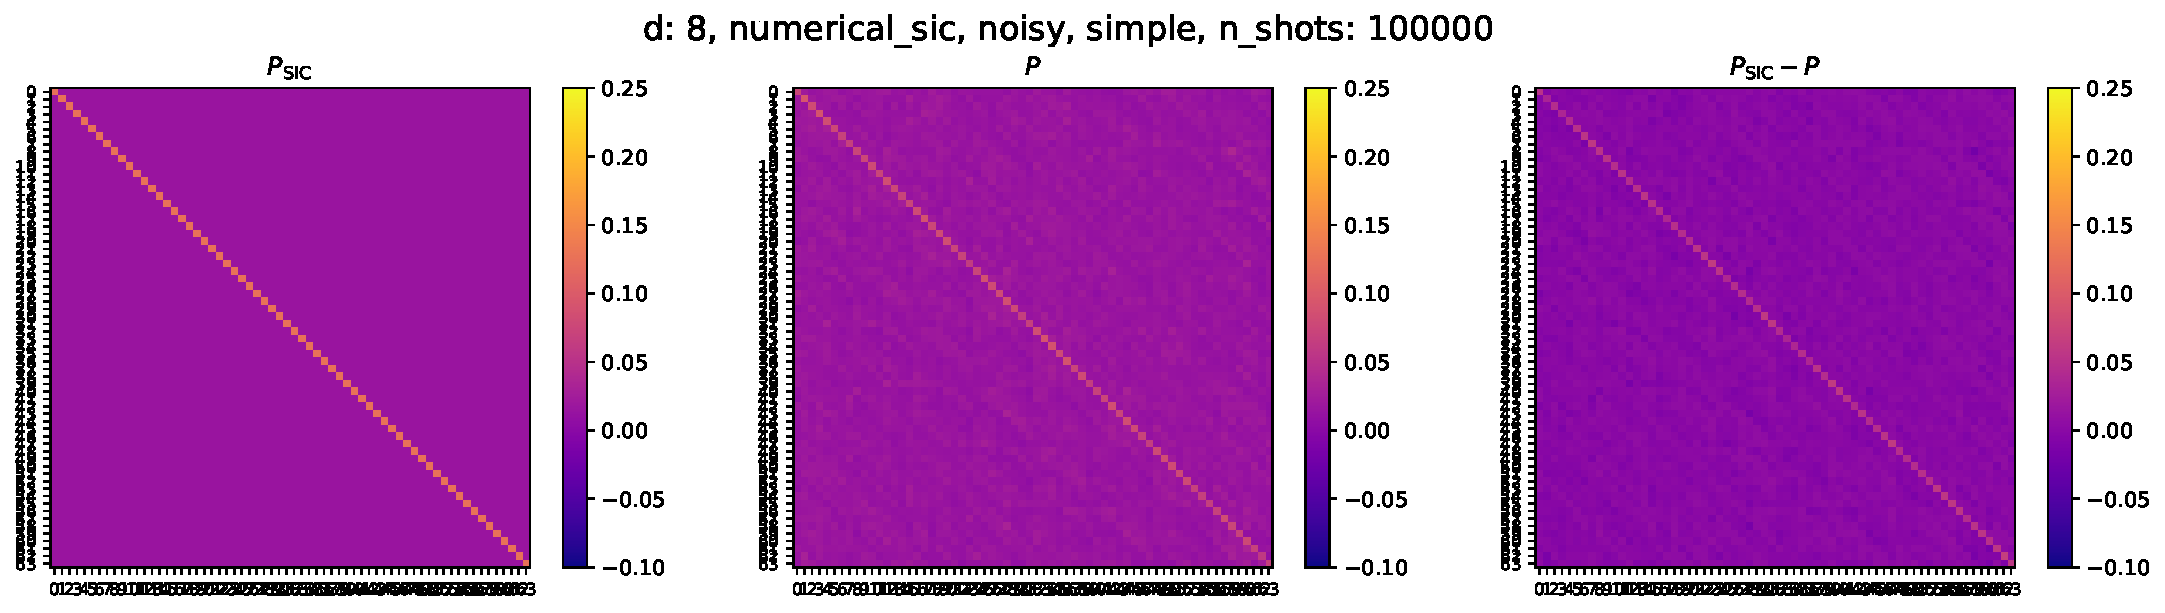
\includegraphics[scale=0.4]{img/P_d8_numerical_sic_noisy_simple_n100000}

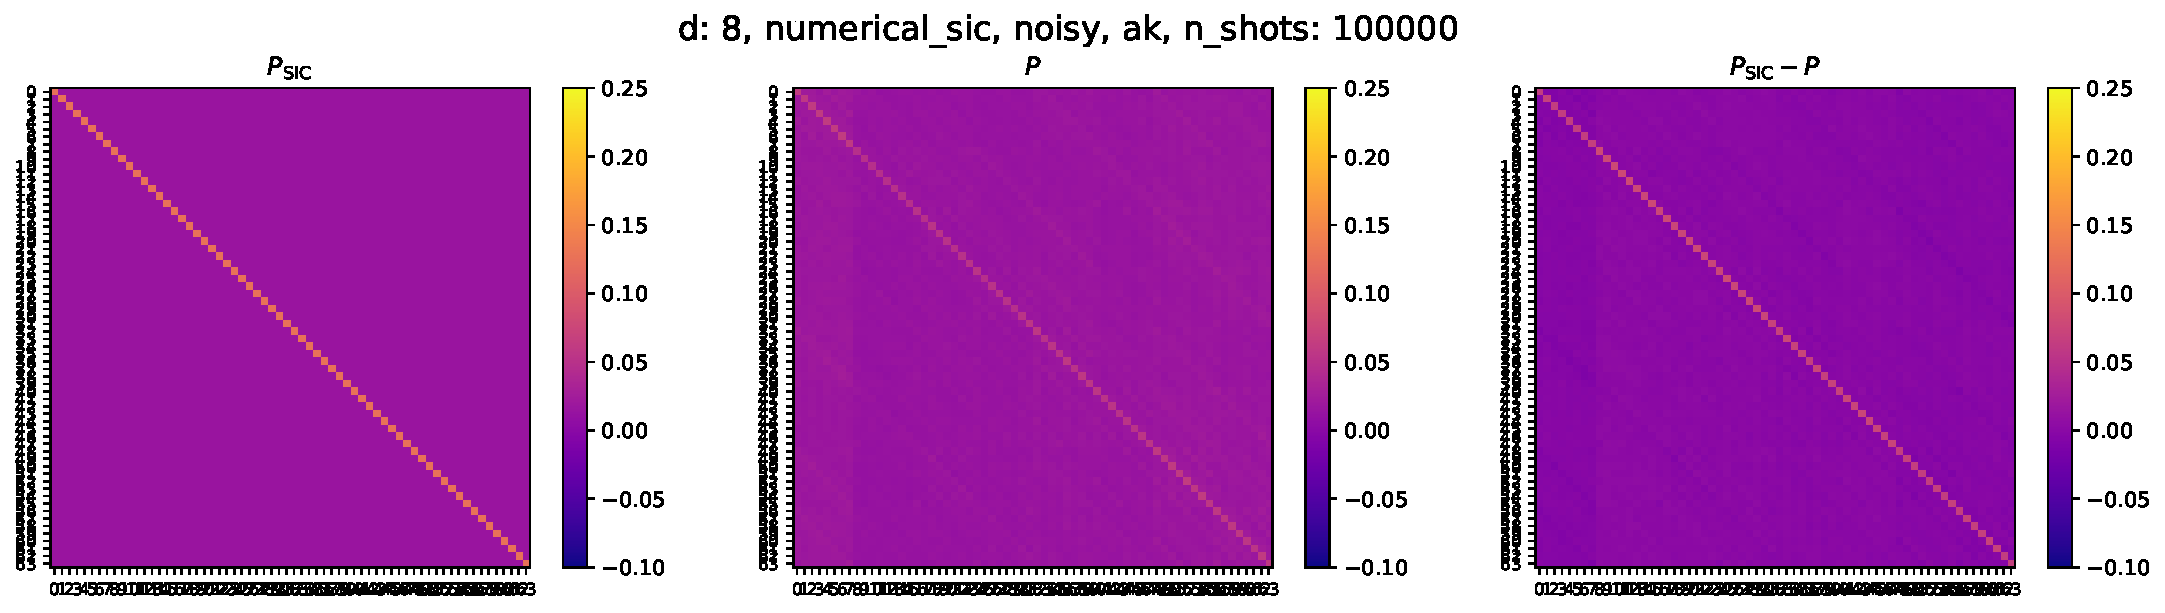
\includegraphics[scale=0.4]{img/P_d8_numerical_sic_noisy_ak_n100000}

\end{center}

\bibliographystyle{plain} 
\bibliography{QuditArthursKelly}

\appendix 

\section{An alternative interpretation}
\label{alt-interpretation}

An interaction with Hamiltonian $A\otimes B$ can be interpreted in two alternative ways,
 \begin{align}
 	e^{i(A \otimes B)}=\sum_a|a\rangle\langle a| \otimes e^{iaB}=\sum_b e^{ibA}\otimes |b\rangle\langle b|,
 \end{align}
where $A=\sum_a a|a\rangle\langle a|$, $B=\sum_b b|b\rangle\langle b|$ are spectral decompositions. In other words, the very same interaction can be interpreted as controlled-$B$ operation, conditional on the observable $A$, or as a controlled $A$-operation, conditional on the observable $B$. In light of this, we may reconsider our Arthurs-Kelly interaction, rewriting it as
\begin{align}
U &= \left(\sum_m I \otimes X^{-m} \otimes |m\rangle_p\langle m|_p	\right)\left(\sum_k X^{-k} \otimes I \otimes |k\rangle\langle k|\right)\\
&=\left(\sum_m I \otimes e^{imP} \otimes |m\rangle_p\langle m|_p	\right)\left(\sum_k e^{ikP} \otimes I \otimes |k\rangle\langle k|\right)\\
&=e^{i(I \otimes P \otimes P)}e^{i(P \otimes I \otimes Q)}\\
&= \left(\sum_m I \otimes |m\rangle_p\langle m|_p\otimes e^{imP} \right)\left(\sum_k |k\rangle_p\langle k|_p \otimes I \otimes e^{ikQ}\right)	\\
&=\left(\sum_m I \otimes |m\rangle_p\langle m|_p\otimes X^{-m} \right)\left(\sum_k |k\rangle_p\langle k|_p \otimes I \otimes Z^{k}\right)\\
&=\sum_{km}|k\rangle_p\langle k|_p \otimes |m\rangle_p\langle m|_p \otimes X^{-m}Z^{k}\\
&=\sum_{km}|k\rangle_p\langle k|_p \otimes |m\rangle_p\langle m|_p \otimes D_{-m,k}.
\end{align}
From this point of view, the Arthurs-Kelly procedure involves coherently applying a WH displacement \emph{on the system} conditional on the momenta of two ancillas. The Kraus operators may be expressed
\begin{align}
K_{xy} &= \Big(\langle x, y| \otimes I\Big)U	\Big(|\gamma\rangle \otimes I\Big)\\
&=\sum_{km}\langle x|k\rangle_p \langle y|m\rangle_p \langle k, m|_p\gamma\rangle D_{-m, k}\\
&=\frac{1}{d}\sum_{km}\omega^{xk+ym}\langle k, m|_p\gamma\rangle D_{-m, k}.
\end{align}
As before, we consider
\begin{align}
K_{00}=	\frac{1}{d}\sum_{mk}\langle k,m|_p\gamma\rangle D_{-m,k},
\end{align}
and then examine $ D_\B{a}^\dagger K_{00}D_\B{a}$. Since $D_\B{a}^\dagger D_{-m,k}D_\B{a} = 	\omega^{xk+ym}D_{-m,k}$, we have
\begin{align}
	D_\B{a}^\dagger K_{00} D_\B{a} &= 	\frac{1}{d}\sum_{mk}\langle k,m|_p\gamma\rangle \omega^{xk+ym}D_{-m,k}=K_{xy},
\end{align}
which again shows that the measurement is WH-covariant. To find the initial state of the ancillas, we use the fact that the WH operators form a basis, so that we can identify
\begin{align}
	\langle k,m|_p\gamma\rangle =\frac{1}{\sqrt{d}}\tr(D_{-m,k}^\dagger \Pi),
\end{align}
or in the discrete position basis
\begin{align}
\label{alt-gamma-expr}
\langle k, m|\gamma\rangle = 	d^{-3/2}\sum_{ab} \omega^{-am+bk}\tr(D_{a,b}^\dagger \Pi).
\end{align}

\section{A slight simplification}
\label{slight-simplification}
Rewriting the Arthurs-Kelly unitary
\begin{align}
U &= \left(\sum_m I \otimes X^{-m} \otimes |m\rangle_p\langle m|_p	\right)\left(\sum_k X^{-k} \otimes I \otimes |k\rangle\langle k|\right)\\
&=(I\otimes I\otimes F) \left(\sum_m I \otimes X^{-m} \otimes |m\rangle\langle m|	\right)(I\otimes I \otimes F^\dagger)\left(\sum_k X^{-k} \otimes I \otimes |k\rangle\langle k|\right),
\end{align}
we notice that strictly speaking we need not apply the final Fourier transform. Indeed, since this operation acts only on the system, and we are measuring the ancillas, applying the final $F$ ought not to affect our probability assignments for the outcomes of the measurement. If we drop the final Fourier transform, we obtain an alternative set of Kraus operators $\{K_{\B{a}}^\prime\}$ such that $E_\B{a}=K_\B{a}^\dagger K_\B{a}=K_\B{a}^{\prime \dagger} K_\B{a}^\prime$. While this simplifies the procedure, the resulting Kraus update is not a L\"uders update, and the post-measurement states will not be proportional to SIC states. 

\section{Addendum on the fiducial preparation}
\label{fiducial-decomposition}

To understand how to prepare the almost flat state $\frac{1}{\sqrt{5+\sqrt{5}}}\begin{pmatrix} \sqrt{2+\sqrt{5}} & 1 & 1 & 1 \end{pmatrix}^T$ from $|0,0\rangle$, we may first rewrite it as
\begin{align}
&a|00\rangle + b|01\rangle + b|10\rangle + b|11\rangle\nonumber	\\
&=|0\rangle\otimes \Big(a|0\rangle+b|1\rangle\Big)+|1\rangle\otimes \Big(b|0\rangle+b|1\rangle\Big)\\
&=\sqrt{a^2+b^2}|0\rangle\otimes \left(\frac{a}{\sqrt{a^2+b^2}}|0\rangle+\frac{b}{\sqrt{a^2+b^2}}|1\rangle\right)+b\sqrt{2}|1\rangle\otimes \left(\frac{1}{\sqrt{2}}|0\rangle+\frac{1}{\sqrt{2}}|1\rangle\right),
\end{align}
for $a=\sqrt{\frac{2+\sqrt{5}}{5+\sqrt{5}}}$, and $b=\sqrt{\frac{1-a^2}{3}}$. We can read off from this expression that we  ought to first transform the first qubit as
\begin{align}
|0\rangle \rightarrow 	\sqrt{a^2+b^2}|0\rangle + b\sqrt{2}|1\rangle,
\end{align}
which, as one can see by matching matrix elements, can be realized by a $y$-rotation with $\theta_1=2\cos^{-1}\left(\sqrt{\frac{1+2a^2}{3}}\right)=2\cos^{-1}\left(\sqrt{\frac{5+\sqrt{5}}{10}}\right)$. In order to prepare the second qubit, we must perform two controlled operations. First, we need to effect the transformation
\begin{align}
|0\rangle \otimes |0\rangle &\rightarrow |0\rangle	\otimes \left(\frac{a}{\sqrt{a^2+b^2}}|0\rangle+\frac{b}{\sqrt{a^2+b^2}}|1\rangle\right),
\end{align}
in such a way that if the first qubit is $|1\rangle$, nothing happens. We may realize this with a controlled $y$-rotation with $\theta_2=2\cos^{-1}\left(\frac{a\sqrt{3}}{\sqrt{1+2a^2}}\right)=2\cos^{-1}\left(\frac{\sqrt{1+\sqrt{5}}}{2}\right)$, but since by convention the rotation is conditional on the control qubit being $|1\rangle$, we must first flip the control, and then flip it back with a Pauli $\sigma_x$ operation. Finally, in order to effect the transformation
\begin{align}
|1\rangle \otimes |0\rangle \rightarrow |1\rangle \otimes \left(\frac{1}{\sqrt{2}}|0\rangle+\frac{1}{\sqrt{2}}|1\rangle\right),
\end{align}
in such a way that if the first qubit is $|0\rangle$, nothing happens, we may use a controlled $y$-rotation with $\theta_3=\pi/2$, which amounts to a controlled-Hadamard transformation. We note that the decomposition of the diagonal phase operation $P$ was provided by Google's Gemini 2.5 Pro.

\section{The meaning of the operator $\B{D}$}
\label{operatorD}

To better understand the structure of $\mathcal{D}$, we can develop it into a more conspicuous form:
\begin{align}
\mathcal{D} &=(I\otimes F^\dagger )\left(\sum_j X^{-j}\otimes |j\rangle\langle j|\right)	\\
&=\sum_j \left[\sum_m |m-j\rangle\langle m|\right]\otimes \left[\frac{1}{\sqrt{d}}\sum_{kl}\omega^{-kl}|k\rangle\langle l|\right]|j\rangle\langle j|\\
&=\frac{1}{\sqrt{d}}\sum_{jkm} \omega^{-jk}|m-j,k\rangle\langle m,j|\\
&=\frac{1}{\sqrt{d}}\sum_{jab} \omega^{-jb}|a,b\rangle\langle a+j,j|\\
&=\frac{1}{\sqrt{d}}\sum_{jab} \omega^{-jb}|a,b\rangle\langle j,j|(X^{-a}\otimes I)\\
&=\frac{1}{\sqrt{d}}\sum_{jab}|a,b\rangle\langle j,j|(Z^{-b}X^{-a}\otimes I)\\
&=\frac{1}{\sqrt{d}}\sum_{ab}|a,b\rangle\sum_j\langle j,j|(D_{a,b}^\dagger\otimes I)\\
&=\frac{1}{\sqrt{d}}\sum_{ab}|a,b\rangle(D_{a,b}|
\end{align}
where we let $a=m-j, b=k$, and $|D_{a,b})$ denotes the row vectorization of $D_{a,b}$. In other words, $\mathcal{D}$ as a matrix simply has $(D_{a,b}|$ as its rows. We then note that the row vectorization of $\Pi$ is precisely
\begin{align} 
|\Pi) &= (\Pi \otimes I)\sum_i |i,i\rangle=\sum_i |\phi\rangle\langle \phi |i\rangle\otimes |i\rangle= |\phi\rangle \otimes \sum_i \langle i|\phi^*\rangle |i\rangle=|\phi\rangle \otimes |\phi^*\rangle,
\end{align}
so that, by the standard vectorization identity $\tr(A^\dagger B) = (A|B)$, 
\begin{align}
	\mathcal{D}\Big(|\phi\rangle \otimes |\phi^*\rangle\Big)=\frac{1}{\sqrt{d}}\sum_{ab}|a,b\rangle (D_{a,b}|\Pi)=\frac{1}{\sqrt{d}}\sum_{ab} \tr(D_{a,b}^\dagger \Pi)|a,b\rangle ,
\end{align}
as desired.

\section{An arbitrary state preparation ansatz}
\label{ansatz_explanation}
\subsection{Block decomposition}
To handle the preparation of arbitrary WH fiducial states in any dimension, we require an ansatz for which it is as easy to prepare the complex conjugate of a state as the original. This is easy enough for a single qubit where we may take $|\psi\rangle = e^{-i\sigma_z\phi/2}e^{-i\sigma_y\theta/2}|0\rangle$ so that, since there is just one relative phase, sending $\phi \rightarrow -\phi$ conjugates the state. \cite{1629135} provides an elegant generalization of this idea for an $n$-qubit state. Beginning, for example, with a $d=2^3$ dimensional state
\begin{align}
|\psi^{(1)}\rangle=\begin{pmatrix} a_1 \\ a_2 \\ a_3 \\ a_4 \\ a_5 \\ a_6 \\ a_7 \\ a_8 \end{pmatrix},
\end{align}
we first interpret $|\psi^{(1)}\rangle$ as the direct sum of four unnormalized qubits,
\begin{align}
|\tilde{\psi_1}^{(1)}\rangle = \begin{pmatrix} a_1 \\ a_2 \end{pmatrix}	&& |\tilde{\psi_2}^{(1)}\rangle = \begin{pmatrix} a_3 \\ a_4 \end{pmatrix}\\
|\tilde{\psi_3}^{(1)}\rangle = \begin{pmatrix} a_5 \\ a_6 \end{pmatrix} && |\tilde{\psi_4}^{(1)}\rangle = \begin{pmatrix} a_7 \\ a_8 \end{pmatrix}.\!\!
\end{align}
Normalizing these qubits and rephasing them so that the first component is real, e.g.,
\begin{align}
|\psi_i\rangle &=  \frac{e^{-i\arg\langle 0|\tilde{\psi_i}\rangle}}{\sqrt{\langle \tilde{\psi_i}|\tilde{\psi_i}\rangle}} |\tilde{\psi_i}\rangle,
\end{align}
we can extract angles
\begin{align}
\theta_i &= 2\arccos\ \langle 0 |\psi_i\rangle 	&& \phi_i = \arg \ \langle 1 |\psi_i\rangle
\end{align}
to obtain  a unitary  $U_i = e^{-i\sigma_z\phi_i/2}e^{-i\sigma_y\theta_i/2}$ so that \begin{align}
U_i^\dagger |\tilde{\psi}_i\rangle = b_i|0\rangle	
\end{align}
for some complex number $b_i$. Doing this for each of the four unnormalized qubits, we obtain four unitaries  $\{U_i^{(1)}\}$ as well as four complex numbers $\{b_i\}$, which we may arrange into a vector:
\begin{align}
	|\tilde{\psi}^{(2)}\rangle = \begin{pmatrix}b_1 \\ b_2 \\ b_3 \\ b_4 \end{pmatrix}.
\end{align}
We then repeat the process, splitting $|\tilde{\psi}^{(2)}\rangle$ into
\begin{align}
|\tilde{\psi_1}^{(2)}\rangle = \begin{pmatrix} b_1 \\ b_2 \end{pmatrix}	&& |\tilde{\psi_2}^{(2)}\rangle = \begin{pmatrix} b_3 \\ b_4 \end{pmatrix},	
\end{align}
from which we obtain $U_1^{(2)}, U_2^{(2)}$, as well as
\begin{align}
|\tilde{\psi}^{(3)}\rangle = \begin{pmatrix} c_1 \\ c_2 \end{pmatrix}.	
\end{align}
Repeating the process yet again, we obtain $U_1^{(3)}$ and $d_1$. In fact, $d_1=e^{i\phi}$ will simply be a phase so that $U_1^{(4)}=e^{i \sigma_z \phi}$. Putting this all together, we have
\begin{align}
|\psi\rangle=\begin{pmatrix}
U_1^{(1)} & & & \\
& U_2^{(1)} & & \\
& & U_3^{(1)} & \\
& & & U_4^{(1)}
 \end{pmatrix}	
 \left[\begin{pmatrix} 
 U_1^{(2)} & \\
	& U_2^{(2)}
 \end{pmatrix} \otimes I_{2^1}\right] \left[U_1^{(3)}U_1^{(4)} \otimes I_{2^2}\right]|0\rangle.
\end{align}
It is instructive to work through the recomposition of the state. First,
\begin{align}
	\Big[U_1^{(4)} \otimes I_4\Big]\Big[|0\rangle \otimes |0\rangle \otimes |0\rangle\Big] = d_1|0\rangle \otimes |0\rangle \otimes |0\rangle.
\end{align}
Then, recalling that we always have $U_i^\dagger |\tilde{\psi}_i\rangle = z_i|0\rangle$ so that $|\tilde{\psi}_i\rangle = z_i U_i |0\rangle$,
\begin{align}
	\left[U_1^{(3)} \otimes I_{4}\right]\Big[d_1|0\rangle \otimes |0\rangle \otimes |0 \rangle\Big] &= |\tilde{\psi}_1^{(3)}\rangle \otimes |0\rangle \otimes |0\rangle= \begin{pmatrix}c_1 \\ 0 \\c_2 \\ 0 \end{pmatrix} \otimes |0\rangle.
\end{align}
Next,
\begin{align}
\left[\begin{pmatrix} 
 U_1^{(2)} & \\
	& U_2^{(2)}
 \end{pmatrix} \otimes I_{2}\right]	\begin{pmatrix}c_1 \\ 0 \\c_2 \\ 0 \end{pmatrix} \otimes |0\rangle&=\begin{pmatrix}  U_1^{(2)}\begin{pmatrix} c_1 \\ 0 \end{pmatrix} \\ U_2^{(2)}\begin{pmatrix} c_2 \\ 0 \end{pmatrix} \end{pmatrix} \otimes |0\rangle
 =\begin{pmatrix}  \begin{pmatrix} b_1 \\ b_2 \end{pmatrix} \\ \begin{pmatrix} b_3 \\ b_4 \end{pmatrix} \end{pmatrix} \otimes |0\rangle
 = \begin{pmatrix} b_1 \\ 0 \\ b_2 \\ 0 \\ b_3 \\ 0 \\ b_4 \\ 0 \end{pmatrix},
\end{align}
and finally,
\begin{align}
\begin{pmatrix}
U_1^{(1)} & & & \\
& U_2^{(1)} & & \\
& & U_3^{(1)} & \\
& & & U_4^{(1)}
 \end{pmatrix}		\begin{pmatrix} b_1 \\ 0 \\ b_2 \\ 0 \\ b_3 \\ 0 \\ b_4 \\ 0 \end{pmatrix}=
 \begin{pmatrix}
 	U_1^{(1)} \begin{pmatrix} b_1 \\ 0 \end{pmatrix} \\ 
 	U_2^{(1)} \begin{pmatrix} b_2 \\ 0 \end{pmatrix} \\ 
 	U_3^{(1)} \begin{pmatrix} b_3 \\ 0 \end{pmatrix} \\ 
 	U_4^{(1)} \begin{pmatrix} b_4 \\ 0 \end{pmatrix} \\ 
 \end{pmatrix}= \begin{pmatrix} a_1 \\ a_2 \\ a_3 \\ a_4 \\ a_5 \\ a_6 \\ a_7 \\ a_8 \end{pmatrix}=|\psi\rangle.
\end{align}
Crucially, just like in the single qubit case, if we negate all the $\phi$'s, we obtain the complex conjugate of our original state. 

\subsection{Performing block-diagonal rotations}

This procedure relies on the ability to perform  block diagonal or \emph{uniformly controlled} rotations. \cite{PhysRevLett.93.130502} proposes a method for doing so. For example, suppose we wish to perform a uniformly controlled-$Z$ rotation, in other words, a block diagonal unitary where each block has the form $R_i=e^{-i\sigma_z \theta_i/2}$ for some angles $\theta_i$. If we are working with $n$ qubits, we must specify $2^{n-1}$ angles. Let
\begin{align}
M_{ij} = 2^{-(n-1)} (-1)^{\vec{b}(j) \cdot \vec{g}(i)}	
\end{align}
be a $2^{n-1} \times 2^{n-1}$ matrix where $\vec{b}(j)$ is the binary vector corresponding to the standard binary representation of the number $j$ and $\vec{g}(i)$ is the binary vector corresponding to the representation of $i$ in the \emph{binary reflected Gray code}\footnote{The binary reflected Grey code provides a binary representation of a number such that two successive numbers differ only by a single bit. It can be easily constructed recursively. Beginning with the 1-bit Grey code $[0,1]$, one obtains the $(n+1)$-bit Grey code by prepending 0's to the $n$-bit code, prepending 1's to the $n$-bit code in the reverse order, and concatenating the two lists. For exaple, the 2-bit code is $[00,01, 11, 10]$, and the 3-bit code is
\begin{align}
[000,001,011,010,110,111,101,100].	
\end{align}}. 
Letting $\vec{\theta}$ be the vector of angles $\{\theta_i\}$, we form
\begin{align}
\vec{\alpha} 	= M \vec{\theta}
\end{align}
to obtain a new set of angles $\{\alpha_i\}$. \cite{PhysRevLett.93.130502}  shows how to perform the uniformly controlled rotation by interleaving single qubit rotations by the $\alpha_i$'s interleaved with \T{CNOT}'s arranged in a particular pattern determined by the binary Gray code: the control wire on the $i$'th \T{CNOT} gate is just the place where the $i$'th and $(i+1)$'th bit strings of the binary reflected Gray code differ. 
\begin{center}
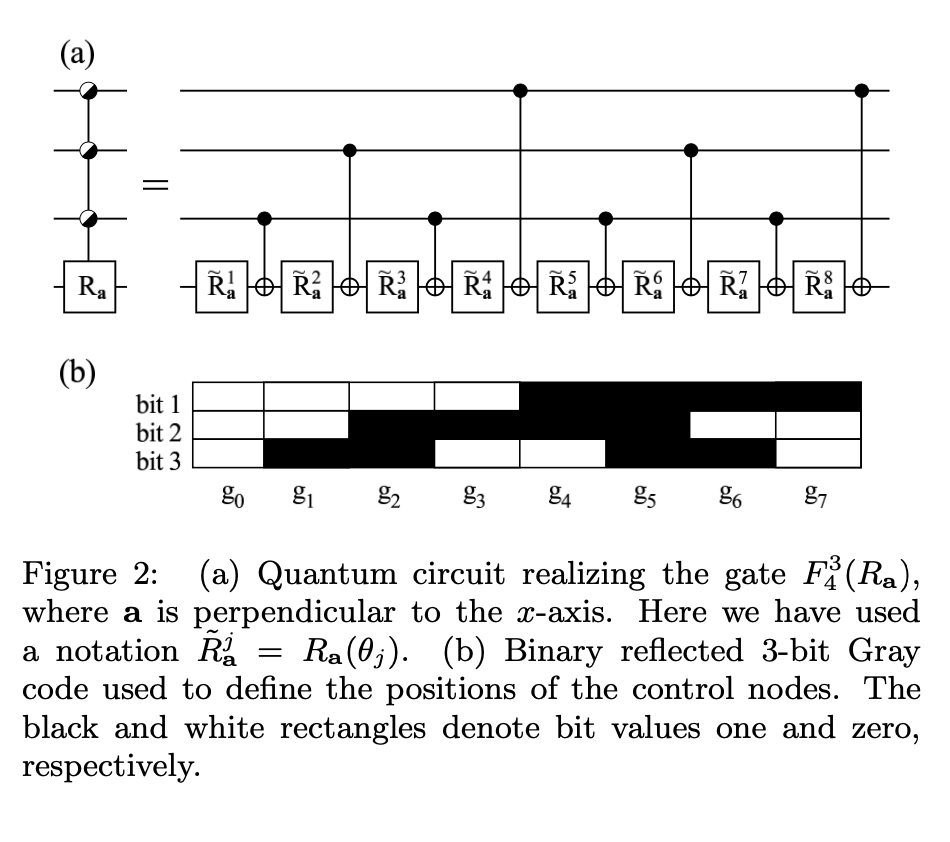
\includegraphics[scale=0.6]{img/uniformly_controlled.png}	.
\end{center}


\section{Noise analysis}

\subsection{Depolarizing $\Phi$}
Let $P =  \frac{1}{d+1}\left(I + \frac{1}{d}J\right)$. Then $\Phi=(d+1)-\frac{1}{d}J$. Depolarizing noise in the states leads to
\begin{align}
P_\alpha &= (1-\alpha) P + \frac{\alpha}{d^2}J	\\
&= \frac{1-\alpha}{d+1}\left(I + \frac{1}{d}J\right)+\frac{\alpha}{d^2}J	\\
&= \frac{1-\alpha}{d+1}I + \frac{\alpha +d }{d^2(d+1)}J.
\end{align}
In the limit of maximum depolarizing noise
\begin{align}
\lim_{\alpha\rightarrow 1} P_\alpha = \frac{1}{d^2}J.	
\end{align}
Up until that point, the reference device is still informationally complete.
Now an $n\times n$ matrix of the form
\begin{align}
M = a I + bJ	
\end{align}
for $a\neq 0$ has an inverse
\begin{align}
M^{-1} = a^{-1}I + n^{-1}((a+nb)^{-1} - a^{-1})J	.
\end{align}
Thus
\begin{align}
\Phi_\alpha = P^{-1}_{\alpha}=\left(\frac{d+1}{1-\alpha}\right)I + \left(1-\frac{d+1}{1-\alpha}\right)\frac{1}{d^2}J.	
\end{align}
In the limit of maximum depolarizing noise, $\Phi_\alpha$ is no longer invertible. From the formula for the inverse, we can see that as $\alpha$ approaches 1, 
\begin{align}
	\lim_{\alpha\rightarrow 1}\left(\frac{d+1}{1-\alpha}\right) = \infty && \lim_{\alpha\rightarrow 1} \left(1-\frac{d+1}{1-\alpha}\right)=-\infty,	\end{align}
that is, the diagonal entries diverge in the positive direction, and the off-diagonal in the negative.

\subsection{Depolarizing state-space}

For simplicity, let us assume depolarization (with parameter $0 \leq \alpha\leq 1 $) of just the SIC measurement itself. The  POVM elements become
\begin{align}
R_i^{(a)}= (1-\alpha)	R_i + \alpha I/d^2,
\end{align}
and 
\begin{align}
P(R_i^{(a)}) = (1-\alpha) P(R_i) + \alpha\left(\frac{1}{d^2}\right):
\end{align}
we simply mix the original probabilities with the flat distribution. If we plug this into the Urgleichung,
\begin{align}
Q(E_i) &= \sum_j P(E_i|R_j)\left[(d+1)P(R_i^{(a)}) - \frac{1}{d}\right]\\
&=\sum_j P(E_i|R_j)\left[(d+1)(1-\alpha) P(R_i) + \alpha\left(\frac{d+1}{d^2}\right) -\frac{1}{d}\right],
\end{align}
we see that if we take the depolarization parameter to be
\begin{align}
\alpha &=\frac{d}{d+1}, 
\end{align}
then
\begin{align}
Q(E_i) &= \sum_j P(E_i|R_j)P(R_j):
\end{align}
the LTP is recovered in the presence of noise. Notice that the most negative a SIC quasiprobability can be is $-\frac{1}{d}$. When $\alpha=\frac{d}{d+1}$, the smallest value a quasiprobability can take is exactly 0. After that point, the quasiprobabilities are just probabilities, as $\alpha$ increases, approaching the flat distribution. Depolarizing noise is picked out as special here since the corresponding measure-and-reprepare SIC channel is itself depolarizing \cite{PhysRevA.100.062327}, and the map to quasiprobabilities is precisely the inverse of this depolarizing channel. Normally applying this inverse takes you out of the $[0,1]$ range, but if you have enough extra depolarization, you can stay inside it. 

Letting
\begin{align}
\rho^{(\alpha)}=(1-\alpha)\rho + \alpha I/d,
\end{align}
we have
\begin{align}
\lVert \rho^{(\alpha)}\rVert	&= \lVert (1-\alpha)\rho + \alpha I/d\rVert\\
&=\sqrt{\tr\left[\Big((1-\alpha)\rho + \alpha I/d\Big)\Big((1-\alpha)\rho + \alpha I/d\Big)\right]}\\
&=\sqrt{(1-\alpha)^2\tr(\rho^2)- \frac{\alpha(\alpha-2)}{d}},
\end{align}
so that, supposing $\rho$ pure,
\begin{align}
\lVert \rho^{(\alpha)}\rVert	&=\sqrt{1+\frac{1}{d}(d-1)(\alpha-2)\alpha}.
\end{align}
If $\alpha=\frac{d}{d+1}$, this becomes
\begin{align}
	\lVert \rho^{(\alpha)}\rVert	&= \frac{\sqrt{d+3}}{d+1}.
\end{align}
The depolarized quantum state-space is then inscribed in a sphere with this radius: this is the largest sphere such that all negativity washes out from the quasiprobabilities. 

Although only when $\alpha = d/(d+1)$ do we recover the exact LTP, we could say that for $d/(d+1) \leq \alpha \leq 1$, the Urgleichung reduces to a classically explicable expression. That said, there's a kind of theoretical assumption here: when the LTP is ``recovered,'' we arrive at an expression containing $P(R_j)$, the ideal probabilities, whereas the sky path probabilities themselves ought to be
\begin{align}
	P(E_i) = \sum_j P(E_i|R_j) P(R_j^{(\alpha)}),
\end{align}
 that is, more depolarized. 
 
 \subsection{The SIC simplex are the quasi-classical states}
 
Since $\Phi=P^{-1}$, $\Phi$ sends MIC probability vectors (the columns of $P$) to the vertices of the simplex (the basis vectors). Since $\Phi$ invertibly maps the reference polytope to the probability simplex, any state outside the polytope will be mapped to a state outside the probability simplex, and thus it must contain quasiprobabilities. It also follows that the only pure states with a properly probabilities as quasiprobabilities are the reference states themselves.

The Euclidean volume of the probability simplex is
\begin{align}
\text{vol}(\Delta)= \frac{d}{(d^2-1)!}.
\end{align}
The Euclidean volume of the SIC simplex is
\begin{align}
\text{vol}(\Delta_{\text{SIC}})&= \frac{d}{(d^2-1)!}\left(\frac{1}{d+1}\right)^{d^2-1}	
\end{align}
Their ratio is
\begin{align}
\frac{\text{vol}(\Delta_{\text{SIC}})}{\text{vol}(\Delta)} = \left(\frac{1}{d+1}\right)^{d^2-1}	.
\end{align}
As $d\rightarrow \infty$, this ratio goes to 0 so that the proportion of quasi-classical states, i.e. states for which the Born rule looks like the LTP, goes to 0. We note that if you consider the sphere in which state space is inscribed (within the probability simplex), under the depolarizing map with $\alpha=d/(d+1)$, this sphere becomes the in-sphere of the SIC simplex.

Meanwhile, the volume of quantum state space itself within the probability simplex is \cite{PhysRevResearch.2.013074}
\begin{align}
\text{vol}(Q)=\sqrt{\frac{(2\pi)^{d(d-1)}}{d^{d^2-2}(d+1)^{d^2-1}}}\frac{\Gamma(1)\cdots \Gamma(d)}{\Gamma(d^2)}	.
\end{align}
(We note that Theorem 2 of the same paper tells us that this volume is the maximum possible among MIC's.) Then
\begin{align}
\frac{\text{vol}(\Delta_{\text{SIC}})}{\text{vol}(Q)}	&= \sqrt{\frac{d^{d^2}}{(d+1)^{d^2-1}(2\pi)^{d(d-1)}}}\frac{1}{\Gamma(1)\dots \Gamma(d)}.
\end{align}




\subsection{Average negativity}
 A non-negative quasi-probability distribution may be interpreted as a distribution over hidden variables. Thus we can ask: how ``quantum'' are we on average? We prepare 1000 random pure states, perform the SIC, and consider the average sum of the negative entries of their quasi-probabilities. On the left, we use the empirical $\Phi=P^{-1}$ to calculate quasi-probabilities. On the right, we use $\Phi_{\text{SIC}}$.	
	\begin{center}
	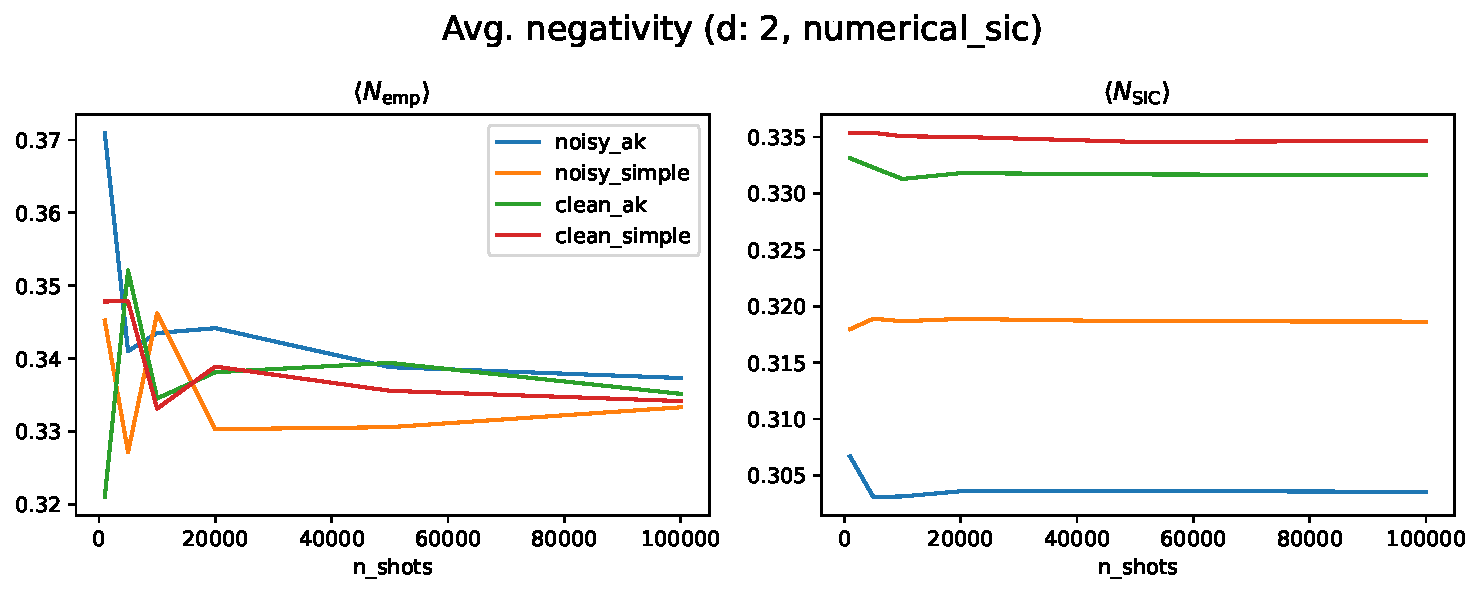
\includegraphics[scale=0.6]{img/avg_neg_d2_numerical_sic}	
	\end{center}

\section{Avoiding intermediate measurement}

The full AK unitary which should act on $|\phi^*\rangle \otimes |\phi\rangle \otimes |\psi\rangle$, where $|\phi\rangle$ is the fiducial and $|\psi\rangle$ is the state to be measured:
\begin{align}
U &= \left(\sum_m I \otimes X^{-m} \otimes |m\rangle_p\langle m|_p	\right)\left(\sum_k X^{-k} \otimes I \otimes |k\rangle\langle k|\right)\left(\sum_j |j\rangle\langle j|\otimes Z^j	\otimes I\right)\Big(I \otimes F^\dagger \otimes I\Big)\\
&=\sum_{jmk} X^{-k}|j\rangle\langle j| \otimes X^{-m}Z^{j}F^\dagger \otimes |m\rangle_p\langle m|_pk\rangle\langle k|\\
&=\sum_{jmk}\omega^{-mk} \ |j-k\rangle\langle j|\otimes X^{-m}Z^{j}F^\dagger \otimes|m\rangle_p\langle k|...
\end{align}

\end{document}